
%--------------------------------------------------------------------
% Document Style
%--------------------------------------------------------------------
\documentclass[12pt]{report}
\usepackage{smu_thesis}
\usepackage{epsf}
\usepackage{amsmath}
\usepackage{graphicx}
\usepackage{verbatim}
\usepackage{epstopdf}
\usepackage{float}
\usepackage{listings}
\usepackage{color}
%\usepackage{algorithm}
%\usepackage{algorithmic}
\usepackage{fancyhdr}
\usepackage{bm}

\definecolor{codegreen}{rgb}{0,0.6,0}
\definecolor{codegray}{rgb}{0.5,0.5,0.5}
\definecolor{codepurple}{rgb}{0.58,0,0.82}
\definecolor{backcolour}{rgb}{0.95,0.95,0.92}

\lstdefinestyle{mystyle}{
	backgroundcolor=\color{backcolour},   
	commentstyle=\color{codegreen},
	keywordstyle=\color{magenta},
	numberstyle=\tiny\color{codegray},
	stringstyle=\color{codepurple},
	basicstyle=\footnotesize,
	breakatwhitespace=false,         
	breaklines=true,                 
	captionpos=b,                    
	keepspaces=true,                 
	numbers=left,                    
	numbersep=5pt,                  
	showspaces=false,                
	showstringspaces=false,
	showtabs=false,                  
	tabsize=2
}

\lstset{style=mystyle}



\linespread{1.6}
%\thesisdraft
\usepackage{hyperref}

\begin{document}

%===================================================================
%   Change information used to create front pages of thesis
%===================================================================
%%
%%  last name, first name, initial
%%
\Name{Lively}{S. David}{} %don't put anything in the last brackets

%%
%% title -- you have up to three lines to specify your title
%% each line should be no more than 48 characters long
%%
\Title{GoLightly: }
{A GPU Implementation of the}
{Finite-Difference Time-Domain Method}
%%
%% previous degress
%%
\DegreeA{B.S.E.E, Southern Methodist University, 2008}
%%
%% degree you are seeking
%%
\DegreeSought{Master of Science}
%%
%% major
%%
\Major{Electrical Engineering}
\University{Southern Methodist University}
\School{Lyle School of Engineering}
%%
%% date the degree will be confered
%%
\DegreeDate{August 1, 2016}
\ThesisDate{August 1, 2016}

%%
%% is this a thesis, dissertation, or something else?
%%
\ThesisType{Thesis}
%%
%% your committee -- the rank of your advisor must be adjusted in
%% smu_thesis.sty if it is not Dr.
%%
\Advisor{Marc Christensen}
\CommitteeMemberA{Professor Ira Greenberg}
\CommitteeMemberB{Dr. Nathan Huntoon}

%===================================================================
%   Create the front pages of the thesis
%===================================================================

 \ApprovalTitlePages

%%
%% include your acknowledgements
%% If no dedication, move Acknowledgement to where dedication is and add to
%% table of contents
%% \addcontentsline{toc}{chapter}{\protect \noindent {ACKNOWLEDGMENTS}}
 \begin{Acknowledgment}
 
I thank my committee for their patience, insight and unfailing encouragement. Without them, this thesis would remain vaporware. Never give up, never surrender!

 \end{Acknowledgment}

%%
%% include your abstract
%%
 \begin{Abstract}
 Traditionally, optical circuit design is tested and validated using software which implement numerical modeling techniques such as Beam Propagation, Finite Element Analysis and the Finite-Difference Time-Domain (FDTD) method.

While effective and accurate, FDTD simulations require significant computational power. Existing installations may distribute the computational requirements across large clusters of high-powered servers. This approach entails significant expense in terms of hardware, staffing and software support which may be prohibitive for some research facilities and private-sector engineering firms.

The application of modern programmable GPUs to problems in scientific visualization and computation has facilitated dramatically accelerated development cycles for a variety of industry segments including large dataset visualization\cite{raycasting}, aerospace\cite{Strzodka2013381} and optical circuit design. GPU-based supercomputers such as National Labs' Summit\cite{nvidiaNationalLabs}, co-designed by NVIDIA and IBM, provide dramatically increased compute capability while using less power and fewer computers. 

The FDTD algorithm maps well to the massively-multithreaded data-parallel nature of GPUs. This thesis explores a GPU FDTD implementation and details performance gains, limitations of the GPU approach, optimization techniques and potential future enhancements. 
 \end{Abstract}

 \PreliminaryPages


% Uncomment to insert a list of symbols from symbols.tex (or elsewhere)
 %\begin{listofsymbols}
 %\input{symbols}
 %\end{listofsymbols}
%%
%% include your dedication
%%
 \Dedicate{To Audrey, Wyatt, Walter and Gwendolyn}
\lstlistoflistings

%===================================================================
%   Begin the body of the thesis
%===================================================================
\begin{thesis}
%===================================================================
%   Chapters are included here
%===================================================================

\chapter{Introduction} \label{ch:introduction}

\begin{figure}[H]
	\centering
	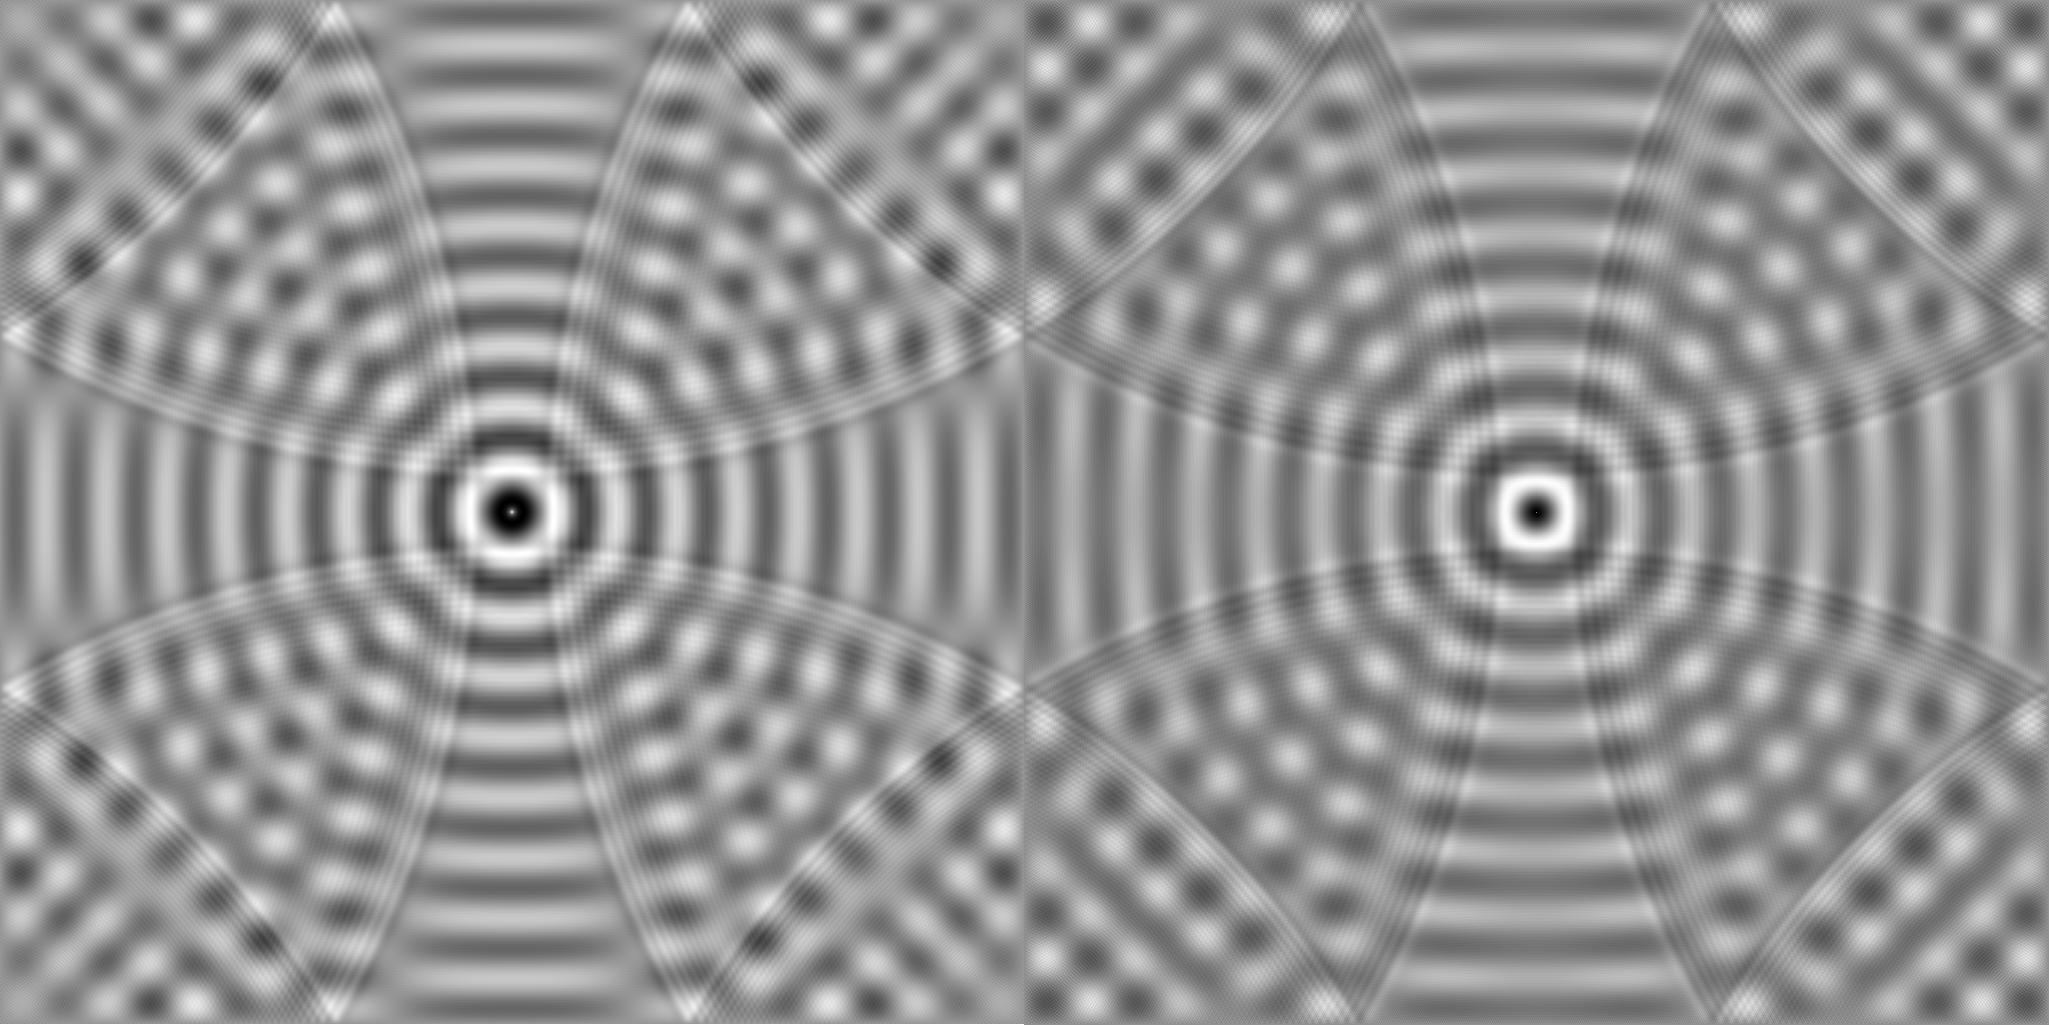
\includegraphics[width=\textwidth,
	keepaspectratio]{point-source-comparison.jpg}
	\caption{GoLightly (left) and Meep (right) result for a point source with Dirlecht boundary conditions}
	\label{fig:pointSourceComparison}
\end{figure}


The FDTD \cite{Yee} algorithm is the underlying mechanism used by many commercial RF simulation packages, as well as open source software such as MIT's Meep\cite{OskooiRo10}. 

Given the computationally-intensive nature of FDTD, organizations requiring simulation of large domains or complex circuits must provide significant resources. These may take the form of leased server time or utilization of an on-site high-performance cluster, amongst other options.

In this thesis, we explore an implementation of FDTD utilizing graphics processing units (GPUs). Initially designed to perform image generation tasks such as those required by games, cinema and related fields, modern versions are well-suited for general computation work. GPUs are now enjoying wide adoption in fields such as machine learning\cite{Raina09largescaledeep} and artificial intelligence\cite{wu2009clustering}, medical research\cite{QIMS1079}, and other areas which require rapid analysis of large datasets.

Even modern consumer-grade GPUs offer thousands or tens of thousands of processing units ("cores"), while high-end CPUs typically offer 4-8 cores. While the two are not interchangeable, some algorithms, such as FDTD, require little or no data interdependence, no branching logic (a severe performance impediment on GPUs) and consist of short cycles of simple operations. The power of the GPU lies in performing these simple operations at large scale, with thousands of threads running in parallel. 

The following sections detail FDTD. Later sections describe a CPU-based implementation (MIT's  Meep simulator), and our GPU-based GoLightly simulator. We verify the GPU solution numerically, and compare performance between CPU- and GPU-based implementations. Finally, we consider future applications and enhancements. 


\section{FDTD Overview}

At it's heart, FDTD expresses Maxwell's equations as a discretized set of time-domain equations\cite{Yee}. These equations describe each electric field component in terms if its orthogonal, coupled magnetic fields, and each magnetic field component as a function of its coupled, orthogonal electric fields.


\subsection{Wave equation}

In a $TM_z$ time domain simulation, wave equation for  $ E_z $ is of the form:

\begin{equation} \label{eq:waveequation} 
\frac{\partial E_z}{\partial t} = K * (\frac{\partial H_x}{\partial y} + \frac{\partial H_y}{\partial x})
\end{equation}

Equation \ref{eq:waveequation} states that the temporal derivative (change in amplitude) of $E_z$ is a function of the $Y$-axis spatial derivative of the $H_x$ field and the $X$-axis spatial derivative of the $H_y$ field.


In order to apply this equation to a computational domain, FDTD defines a cell-based discretization strategy.

\subsection{Yee Cell}

Yee \cite{Yee} defines a computational unit known as a "cell." The cell describes how each field component within a domain is related to it's coupled fields. For instance, in a 2D $TM_z$ simulation, $E_Z$ depends on adjacent $H_y$ and $H_x$ components. The cell format used in such a simulation is of the form shown in \ref{fig:yeecell}.

\begin{figure}[H]
	\centering
	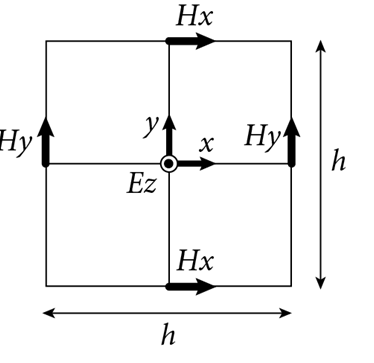
\includegraphics{yee-cell-ez.png}
	\caption{2D $TM_Z$ Yee Cell}
	\label{fig:yeecell}
\end{figure}

More formally, we may expand the $E_Z$ wave equation, arriving at:

\begin{equation} \label{eq:ezupdate}
{E_z}_{i,j}^{t} = C_a * {E_z}_{i,j}^{t-1} 
+ C_b * ({H_x}_{i,j+\frac{1}{2}}^{t-\frac{1}{2}} - {H_x}_{i,j-\frac{1}{2}}^{t-\frac{1}{2}})
+ C_b * ({H_y}_{i+\frac{1}{2},j}^{t-\frac{1}{2}} - {H_xy}_{i-\frac{1}{2},j}^{t-\frac{1}{2}})
\end{equation}

Similarly, the equations for the coupled fields $H_x$ and $H_y$ may be expressed as:
\begin{equation} \label{eq:hxupdate}
{H_x}_{i,j}^t = D_a * {H_x}_{i,j}^{t-1} + D_b * (
{E_z}_{i,j+\frac{1}{2}}^{t-\frac{1}{2}} 
-
{E_z}_{i,j-\frac{1}{2}}^{t-\frac{1}{2}}
)  
\end{equation}

\begin{equation} \label{eq:hyupdate}
{H_y}_{i,j}^t = D_a * {H_y}_{i,j}^{t-1} + D_b * (
{E_z}_{i+\frac{1}{2},j}^{t-\frac{1}{2}} 
-
{E_z}_{i-\frac{1}{2},j}^{t-\frac{1}{2}}
)  
\end{equation}


%\begin{table}[ht]
%	\caption{FDTD Coefficients}
%	\centering
%	\begin{tabular}{c c c}
%		\hline\hline
%		Symbol & Value & Meaning \\
%		\hline
%		$C_a$ & & \\
%		$C_b$ & & \\
%		$D_a$ & & \\
%		$D_b$ & & \\
%		\hline
%	\end{tabular}
%	\label{table:fdtdcoefficients}
%\end{table}













\chapter{Device Architecture} \label{ch:device architecture}

CPUs and GPUs each offer advantages for different computational tasks. Multi-core CPUs offer independent cores which are effectively discrete processors. GPUs, however, offer large-scale parallelization, but require strong data and code coherence in order to achieve acceptable performance.


\section{CPU}

Users typically run many different applications in parallel: a web browser, music player, word processor and email client are a common combination.

In a modern multi-core CPU, each core provides a dedicated ALU and register set. This allows each core to operate as an independent device. This architecture is advantageous when the device is required to perform disparate operations.

Each ALU performs the same operation at the same time, indicating that the additional ALUs are redundant. Thus, the flexible, general-purpose nature of a CPU becomes a limitation when within the context of FDTD.

\section{GPU}

Unlike CPUs, GPUs are capable of running thousands of threads in parallel using a SIMD (single-instruction, multiple-data) model. This architecture is allows rapid processing of large datasets wherein each datum exhibits little or no interdependence. 

This independence is crucial to performant GPU-based applications, as detailed in \autoref{sec:simd}.

\subsection{SIMD}\label{sec:simd}

In a SIMD\cite{Massingill:2007:SAP:1772070.1772078} architecture, a core may consist of a single ALU, with multiple register banks. Separate "threads" load different data into dedicated register banks. The ALU executes identitical operations on all registers simultaneously. In this way, each register bank is analagous to a CPU "thread." However, since the same instruction must be executed on all register sets at every step, this design is less flexible than a system where each core is truly independent. 

That said, the approach provides some benefits, including:

\begin{itemize}
	\item Fewer components are required per core since fewer ALUs are required. Leads to reduced die space requirements.
	\item Better code caching. A single ALU, and corresponding cache, are used for many threads, eliminating the need to load or monitor code cache behavior per thread.
\end{itemize}








\chapter{FDTD} \label{ch:fdtd}


FDTD expresses Maxwell's equations as a set of discretized time-domain equations\cite{Yee}. These equations describe each electric field component in terms if its orthogonal, coupled magnetic fields, and each magnetic field component as a function of its coupled electric fields.


\section{Wave equation}

The TM wave equation for  $E_z$, $H_x$, and $H_y$ are of the form:

\begin{equation} \label{eq:waveequation} 
\frac{\partial E_z}{\partial t} = K * (\frac{\partial H_x}{\partial y} + \frac{\partial H_y}{\partial x})
\end{equation}

\begin{equation}
\frac{\partial H_x}{\partial t} = K * (\frac{\partial E_z}{\partial y})
\end{equation}

\begin{equation}
\frac{\partial H_y}{\partial t} = K * (\frac{\partial E_z}{\partial x})
\end{equation}

These equations state that the temporal derivative of a field is a function of the sum of the spatial derivatives of the coupled orthogonal fields.

In order to apply these equations to a computational domain, FDTD defines discretization strategies for simulated time and space. The simulation domain is divided into cells, and each frame is updated using a fixed time step derived from parameters such as source wavelength and simulation dimensionality.

\section{Yee Cell}

Yee \cite{Yee} defines a computational unit known as a "cell." The cell describes how each field component within a domain is related to it's coupled fields. For instance, each $E_Z$ field component depends on adjacent $H_y$ and $H_x$ components. The cell format used in such a simulation is of the form shown in \autoref{fig:yeecell}.

\begin{figure}[H]
	\centering
	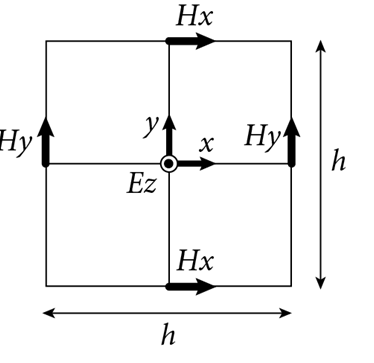
\includegraphics{yee-cell-ez.png}
	\caption{2D $TM_Z$ Yee Cell}
	\label{fig:yeecell}
\end{figure}

More formally, we may expand the $E_Z$ wave equation, arriving at:

\begin{equation} \label{eq:ezupdate}
{E_z}_{i,j}^{t+1} = C_a * {E_z}_{i,j}^{t} 
+ C_b * ({H_x}_{i,j+\frac{1}{2}}^{t+\frac{1}{2}} - {H_x}_{i,j-\frac{1}{2}}^{t+\frac{1}{2}})
+ C_b * ({H_y}_{i+\frac{1}{2},j}^{t+\frac{1}{2}} - {H_xy}_{i-\frac{1}{2},j}^{t+\frac{1}{2}})
\end{equation}

Similarly, the 2D equations for the coupled fields $H_x$ and $H_y$ may be expressed as:

\begin{equation} \label{eq:hxupdate}
{H_x}_{i,j}^{t+1} = D_a * {H_x}_{i,j}^{t} + D_b * (
{E_z}_{i,j+\frac{1}{2}}^{t+\frac{1}{2}} 
-
{E_z}_{i,j-\frac{1}{2}}^{t+\frac{1}{2}}
)  
\end{equation}

\begin{equation} \label{eq:hyupdate}
{H_y}_{i,j}^{t+1} = D_a * {H_y}_{i,j}^{t} + D_b * (
{E_z}_{i+\frac{1}{2},j}^{t+\frac{1}{2}} 
-
{E_z}_{i-\frac{1}{2},j}^{t+\frac{1}{2}}
)  
\end{equation}

\iffalse
From Nathan:

You need to expand this a fair amount more.  You need to at minimum define all of the terms in these equations.  A paragraph or two on how a full domain is discritized, and how a simulation steps in 1/2 detla T steps is important.  

This will be important in the discussion between CPU and GPU architectures as you want to list how with FDTD you calcuate an entire time step, or 'frame' over the entire phyisical domain before moving on to the next frame.  You can state here how the updates of frames are independent of other calculations done during that same frame
\fi

\begin{table}[h!]
	\centering
	\caption{FDTD Equation Terms}
	\label{tab:modelColorComponentUsage}
	\begin{tabular}{l | c | l}
		Symbol	& Definition & Description \\
		\hline				\\										 	 
		$dx$ 	& $\frac{\lambda}{10}$ 			& Spatial step as a function of max source  fundamental frequency 					\\
		$dt$ 	& $\frac{dx}{\sqrt{n}} * 0.9$		& Time step between frame updates, where $n$ is the domain dimensionality \\		$C_a$	& $\frac{1}{\epsilon_0}$ & Permittivity of free space	\\
		$C_b$	& $\frac{dt}{dx}  \frac{1}{\epsilon} $ & Permittivity at the location $i,j$\\
		$D_a$	& $\frac{1}{\mu_0}$	& Permeability of free space \\
		$D_b$	& $\frac{dt}{dx}\frac{1}{\mu}$	& Permeability at the location $i,j$\\
		$i$, $j$ 	& &	Field element location within the domain  \\
		$t$   	& &	Current time step ($t_E = t_H \frac{+}{-}\frac{1}{2}$) \\
		$E_Z$ 	& & Electric field amplitude in $Z$ \\
		$H_X$ 	& & Magnetic field amplitude in $X$ \\
		$H_Y$	& & Magnetic field amplitude in $Y$ \\
	\end{tabular}
\end{table}

Since Maxwell's equations are scale-invariant, GoLightly substitutes 1 for constants such as $C$, $\mu_0$ and $\epsilon_0$. The $\frac{0.9}{\sqrt{2}}$ scalar in $dt$ prevents aliasing, and corrects for simulation dimensionality\footnote{This value should be $\frac{0.9}{\sqrt{n}}$, where $n$ is 3 for a 3D domain, 2 for a 2D domain and 1 for a 1D domain.} 

In equations \ref{eq:ezupdate}, \ref{eq:hxupdate} and \ref{eq:hyupdate}, note that each $E_{i,j}^{t+1}$ field update depends only upon the previous $E$ value ($E_{i,j}^{t}$), and the previous adjacent $H$ values ($H_X^{t+\frac{1}{2}}$ and $H_Y^{t+\frac{1}{2}}$). This independence allows each field component to be updated without regard for any other value in the same field.   

\clearpage

\section{Leap Frog: Stepping in Space and Time}

In equations \ref{eq:ezupdate}, \ref{eq:hxupdate} and \ref{eq:hyupdate}, note the presence of a "half step" in time ($F^{t + \frac{1}{2}}$) and space $F_{i \frac{+}{-}\frac{1}{2},j \frac{-}{+}\frac{1}{2}}$.

This $t\frac{+}{-}\frac{1}{2}$ represents the temporal step size between an $E$-field update and the next $H$-field update,and visa-versa. Similarly, the spatial offset $x\frac{+}{-}\frac{1}{2}$ represents the distance between an $E$-field component and its adjacent, interdependent $H$ values.


\begin{figure}[H]
	\centering
	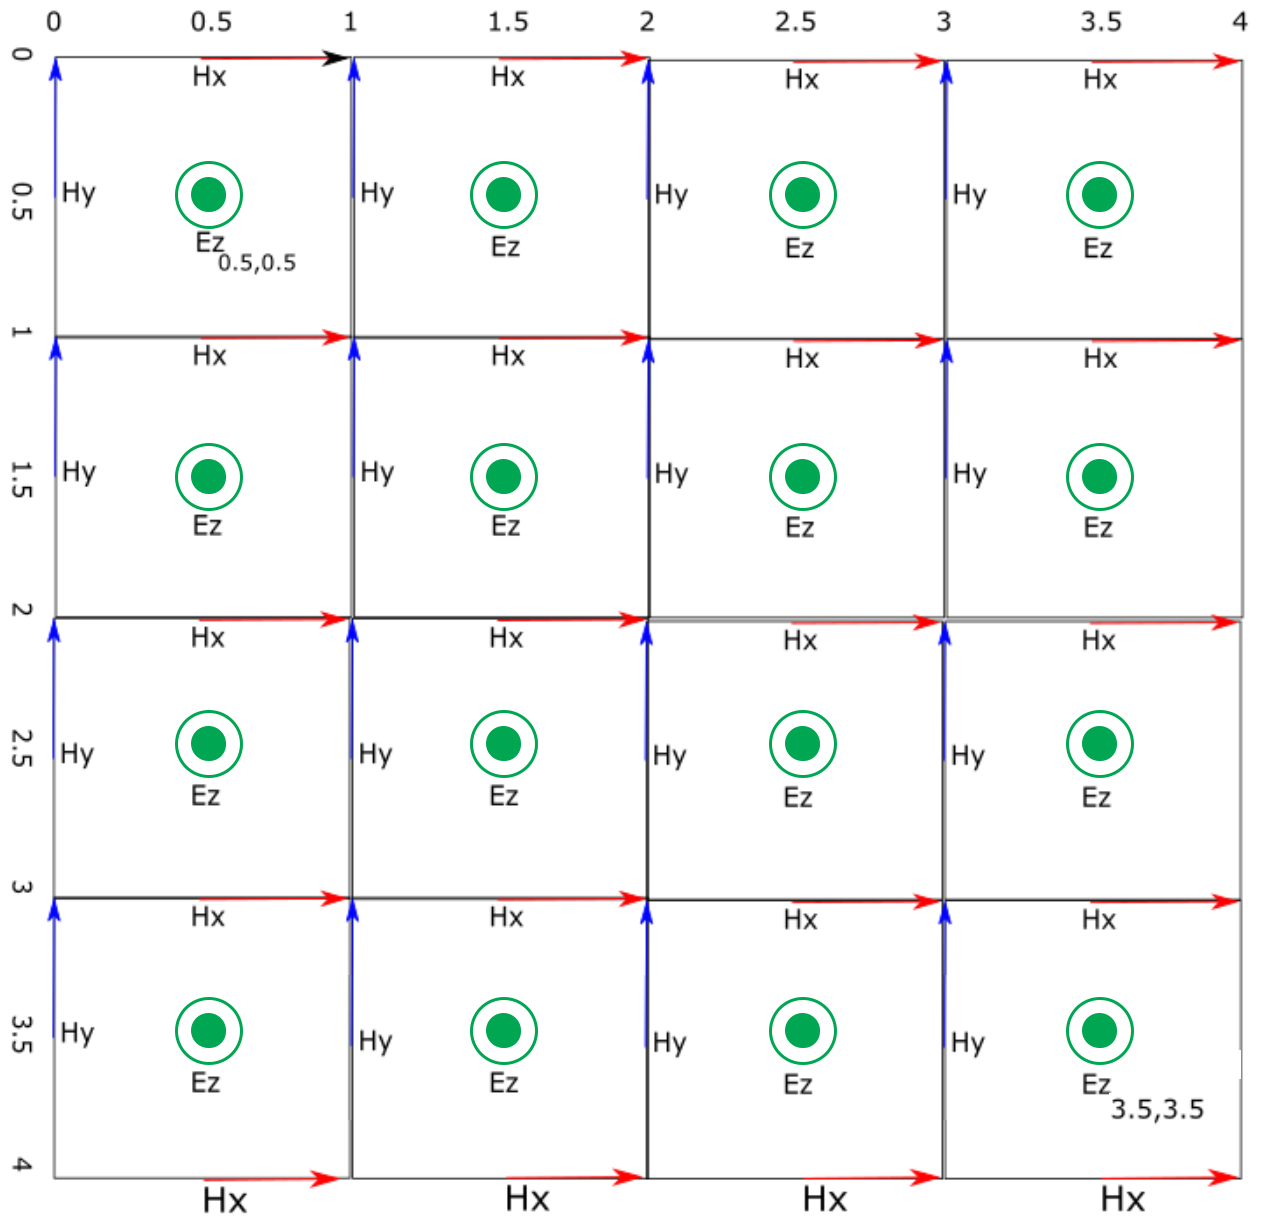
\includegraphics[width=15cm,keepaspectratio]{YeeMesh.png}
	\caption{4x4 Yee Lattice}
	\label{fig:yeeLattice}
\end{figure}

The spatial relationship between $E$ and $H$ grids is illustrated in the Yee lattice in \autoref{fig:yeeLattice}. Note that each $E_Z$ component is in the middle of a cell, at the $(i + \frac{1}{2}, j + \frac{1}{2})$ position where ($i,j$) is  the upper-left corner of the cell. $H$ components, however, are positioned at integer coordinates.

This arrangement reflects the manner in which a wave will propagate through the domain. In the half time step between $E$ and $H$ updates, the wave moves one half-cell. If the $E$ and $H$ components were coincident, the simulation would degrade to a large collection of individual, disjoint points rather than a discretized, connected domain.


\section{Boundary Conditions}

Recall the $H_Y$ update equation \autoref{eq:hyupdate}, and note that it depends on two adjacent $E_Z$ values on the $X$ axis. The finite grid does not contain enough information to update the $H$ values that lie on the edge of the domain. For instance, ${H_Y}_{0,\frac{1}{2}}$ requires ${E_Z}_{\frac{1}{2},\frac{1}{2}}$ and \bm{${E_Z}_{-\frac{1}{2},\frac{1}{2}}$}.

Since the position $(-\frac{1}{2},\frac{1}{2})$ does not exist, the simulator cannot update this value. The simulator must take this case into account by implementing a boundary condition, or the wave will reflect from the boundaries. 

We implement the Perfectly Matched Layer (PML) as described in \cite{BERENGER1994185}. A detailed explanation of PML is beyond the scope of this thesis. In practice, PML adds imaginary hyperplanes orthogonal to each field in the simulation. In the boundary regions, power couples between $E$ and $H$ as expected, but \emph{also} couples into those hyperplanes. Unlike the $E$ and $H$ interdependence, the transfer is one-way. Cells in the PML hyperplanes contain non-physically realizable materials which force the coupled power to decay over a number of layers. In our implementation, we use 10 PML layers as experimentation showed this to provide the most satisfactory results.



\section{FDTD in SIMD}

FDTD's leap-frog update method, whereby E fields and H fields are successively calculated, is well-suited to a GPU implementation. E field values depend on adjacent H field values, and visa-versa. Since the E-field update equation requires knowledge only of the H field state and previous E field state, each field component can be calculated independently with no opportunity for a pipeline stall or race condition. 



\chapter{Meep} \label{ch:meep}

Meep\cite{OskooiRo10} is a full-featured, open-source simulator produced by the Massachusetts Institute of Technology. In addition to its core FDTD-based simulation engine, it provides a scripting interface for defining models and simulation parameters, recording results, and other tasks.  





\section{Modeling}

\iffalse

While I may agree, you need to keep they hyperbole and sarcasm out.  You should re-write this section to state what Meep is, how it is used, and how you made use of some of it's features.  You can also look up how many citations it has (on their website) to showcase that it's widely used and trusted making it a valid point of comparison 
\fi

One limitation of Meep is it's use of an obscure, uncommon scripting language known as SCHEME. Models are defined in terms of constructive solid geometry (CSG) commands, whereby the user describes their model in terms of boolean operations and regular polyhedra. 

While adequate for simple models, constructing an arbitrarily-shaped or dynamic structure in this way may be difficult. In practice, proprietary software may be used to convert more complex model definitions into a format usable by Meep.

It is worth noting that Meep provides a "material function" capability. This allows the user to dynamically determine the material properties of a point in space using their own algorithm rather than defining their model using CSG. However, to take advantage of this capability, the user must employ additional software or custom programming. This further increases the complexity of an already-complicated system. 



\section{Performance}

Meep is a mature, highly-optimized suite of tools. It scales well across multiple machines, relying on the MPI protocol to keep nodes within a simulation cluster in sync. 

While performant when compared to other FDTD software, Meep suffers from the same architecture-imposed limitations of all CPU-based implementations. The limited number of processing cores available on a general-purpose CPU restricts the number of data points that can be be processed within a given time frame. This problem can be solved by provisioning additional computers which would run in parallel, distributing the computational load evenly across the resulting cluster.

This sort of cluster configuration incurs its own overhead. Although a domain may be divided into discrete parts and distributed across cluster nodes, FDTD boundary conditions require that, at some point, parts of the divided domain must be exchanged between nodes to maintain continuity. This necessitates installation of a high-speed local network and supporting hardware. 







\chapter{GoLightly} \label{ch:golightly}

GoLightly is the GPU-based FDTD simulator application that is the focus and product of this thesis. Written using a combination of C++, CUDA and OpenGL, it provides a lightweight yet complete FDTD solution.

\section{Goals}

GoLightly is intended to address deficiencies common to CPU-based solutions. In particular, it is designed to be fast, friendly and portable.


\begin{itemize}
	\item Fast. An iterative design process requires rapid feedback from the simulator. Long simulation times necessitated by existing solutions inhibit this process.
	\item Friendly. Definition of models and other simulation parameters should not require expertise in software development or quasi-proprietary scripting languages. 
	\item Portable. Ideally, the simulator should run on a high-end consumer grade laptop and support the most common desktop operating systems (Microsoft Windows and Apple OS X).  
\end{itemize}

To meet those goals, GoLightly takes advantage of the programmable GPU available in common desktop and laptop computers, resulting in a dramatic speedup. Rather than relying on a proprietary model definition language or obscure, limited scripting system, we use industry-standard image and geometry file formats so that models may be defined using robust, familiar, readily-available tools. By building the software specifically for Microsoft Windows, we ensure that it is compatible with the most common desktop operating system. 

\section{Architecture}

GoLightly comprises three primary application blocks:

\begin{itemize}
	\item Model Processor \ref{sec:modelProcessor}
	\item Simulator \ref{sec:simulator}
	\item Visualizer \ref{sec:visualizer}
\end{itemize}

\section{Model Processor}\label{sec:modelProcessor}

The model processor (MP) is responsible for initialization of the simulator. When launching the simulator, a domain size and image file, containing a coded image of the desired dielectric, as well as a max $\epsilon$ are specified.

\begin{table}[h!]
	\centering
	\caption{Model processor inputs}
	\label{tab:modelProcessorInputs}
	\begin{tabular}{l | l | l | l}
		Symbol	& Data Type & Meaning & Typical value				\\
		\hline														\\
		Width	& int 		& Domain size in X & 1024				\\
		Height	& int 		& Domain size in Y & 1024				\\
		Media	& float 	& $\epsilon_{max}$ & 9						\\
		Model	& string	& Model definition stored as a bitmap & filename
	\end{tabular}
\end{table}

The MP allocates arrays to hold the dielectric properties for each Yee cell. These arrays are of the same dimensions as the domain, which may be different than the dimensions of the model. 

Once the model image is loaded, the MP iterates through each element in the dielectric array. (See \autoref{listing:modelFromImage})

For each element:

\begin{enumerate}
	\item Determine the normalized texel coordinate that corresponds to the current cell position	
	\item Read the red (R), green (G) and blue (B) color components from the image
	\item If $R > 128$, this texel is part of a source. Add the cell to the list of sources
	\item If $G > 0$, this texel has non-unity dielectric. Set ${C_b}_{i,j} = \epsilon_{max} * \frac{G}{255.0}$
	\item If $B > 0$, this texel is part of a monitor. Add its position to the monitor definition with ID = $B$
\end{enumerate}

\lstinputlisting[language=c++,caption=Generating a model from an image]{model-from-image.cpp}\label{listing:modelFromImage}

Once the dielectric, sources and monitors are derived from the model image, the model processor transfers control to the simulator.

\section{Simulator}\label{sec:simulator}

The simulator block implements the FDTD algorithm. Given the dielectric, source and monitor configurations from the model processor, the simulator initializes the GPU, transfers required data from host memory to the GPU, and begins the simulation loop.

In addition to the dielectric and field arrays, the simulator generates a  descriptor (\autoref{listing:fieldDescriptor}) for each field that will be updated. This structure is used by the kernels to assist in handling boundary conditions (PML) and other housekeeping duties. A similar, more compact  descriptor (\autoref{listing:deviceFieldDescriptor}) is generated from the host descriptor and passed to the kernels.

\lstinputlisting[language=c++,caption=Host Field Descriptor structure]{fieldDescriptor.cpp}\label{listing:fieldDescriptor}

\lstinputlisting[language=c++,caption=Device Field Descriptor]{deviceFieldDescriptor.cpp}\label{listing:deviceFieldDescriptor}

For each loop iteration, the simulator launches a CUDA kernel to update all $E$ fields. Once the $E$ update is complete, the simulator launches kernels to update all $H$ fields.

The three kernels required for a $TM_Z$ simulation are detailed below:

\lstinputlisting[language=c++,caption=CUDA kernel for updating $E_Z$]{cu_update_ez.cpp}\label{listing:updateEzCpp}

The majority of each kernel's source performs setup and bounds checking tasks. In each kernel, the FDTD equation implementation can be isolated to one or two lines of code.

For example, the line (from the $E_Z$ update kernel),

\begin{lstlisting}
	Ez->Data[center] = CA * Ez->Data[center] + cb * (dhy - dhx) + cb * (ezxPsi - ezyPsi);
\end{lstlisting}

corresponds to the FDTD $E_Z$ equation. (See \autoref{eq:ezupdate})

\lstinputlisting[language=c++,caption=CUDA kernel for updating $H_X$]{cu_update_hx.cpp}\label{listing:updateHxCpp}

\lstinputlisting[language=c++,caption=CUDA kernel for updating $H_Y$]{cu_update_hy.cpp}\label{listing:updateHyCpp}

Note that all $E$ updates occur simultaneously, as do all H fields. However, given the dependence between the $E$ and $H$ fields, the $E$ field update kernels must complete before the $H$ fields are updated.

The simulator repeats this operation until the application is closed, or the desired number of frames are completed. 

Finally, the completed field arrays are copied to the host from the GPU, and saved to disk in bitmap and CSV format for later analysis. 

\section{Visualizer}\label{sec:visualizer}

If enabled \footnote{The visualizer requires some GPU overhead. As such, its use may affect simulator performance.}, the visualizer application block provides interactive display of the simulation. 

When running a simulation, the user may optionally specify a visualizer update frequency, indicating the number of simulation frames that should complete between visualizer updates. This aids in reducing the visualizer's performance impact.

A window and OpenGL context are created using GLFW and the glLoadGen OpenGL extension loader. An OpenGL pixel buffer object (PBO) is allocated to contain a copy\footnote{The PBO may be of different dimensions than the simulation domain. Since the PBO is used only for visualization, it is not necessary for it to contain the full-resolution field.} of the field that the user wishes to see\footnote{The visualizer provides the ability to dynamically select which field(s) should be displayed}. 

The visualizer also creates a screen-aligned quad on which the field texture will be rendered, and allocates a texture object which is then bound to the PBO\autoref{fig:visualizerUpdatePipeline}.

\begin{figure}[H]
	\centering
	\includegraphics[  width=0.5\textwidth,
	keepaspectratio]{visualizerPipeline.png}
	\caption{Visualizer Update Pipeline}
	\label{fig:visualizerUpdatePipeline}
\end{figure}



After the required number of frames have been completed, the visualizer launches a CUDA kernel which samples the selected field and populates the PBO. 

\lstinputlisting[language=c++,caption=CUDA kernel for updating visualizer pixel buffer object]{cu_visualizer_update.cpp}

A completed PBO is bound to a uniform input for a shader (\autoref{listing:basicVertGlsl},\autoref{listing:basicFragGlsl}) which renders the texture to the visualizer window. 

\lstinputlisting[language=c++,caption=GLSL Vertex Shader]{basic_vert.glsl}\label{listing:basicVertGlsl}
\lstinputlisting[language=c++,caption=GLSL Fragment Shader]{basic_frag.glsl}\label{listing:basicFragGlsl}

This process runs continuously. However, the texture is only updated at the frequency requested by the user when the simulation was launched. 

\begin{figure}[H]
	\centering
	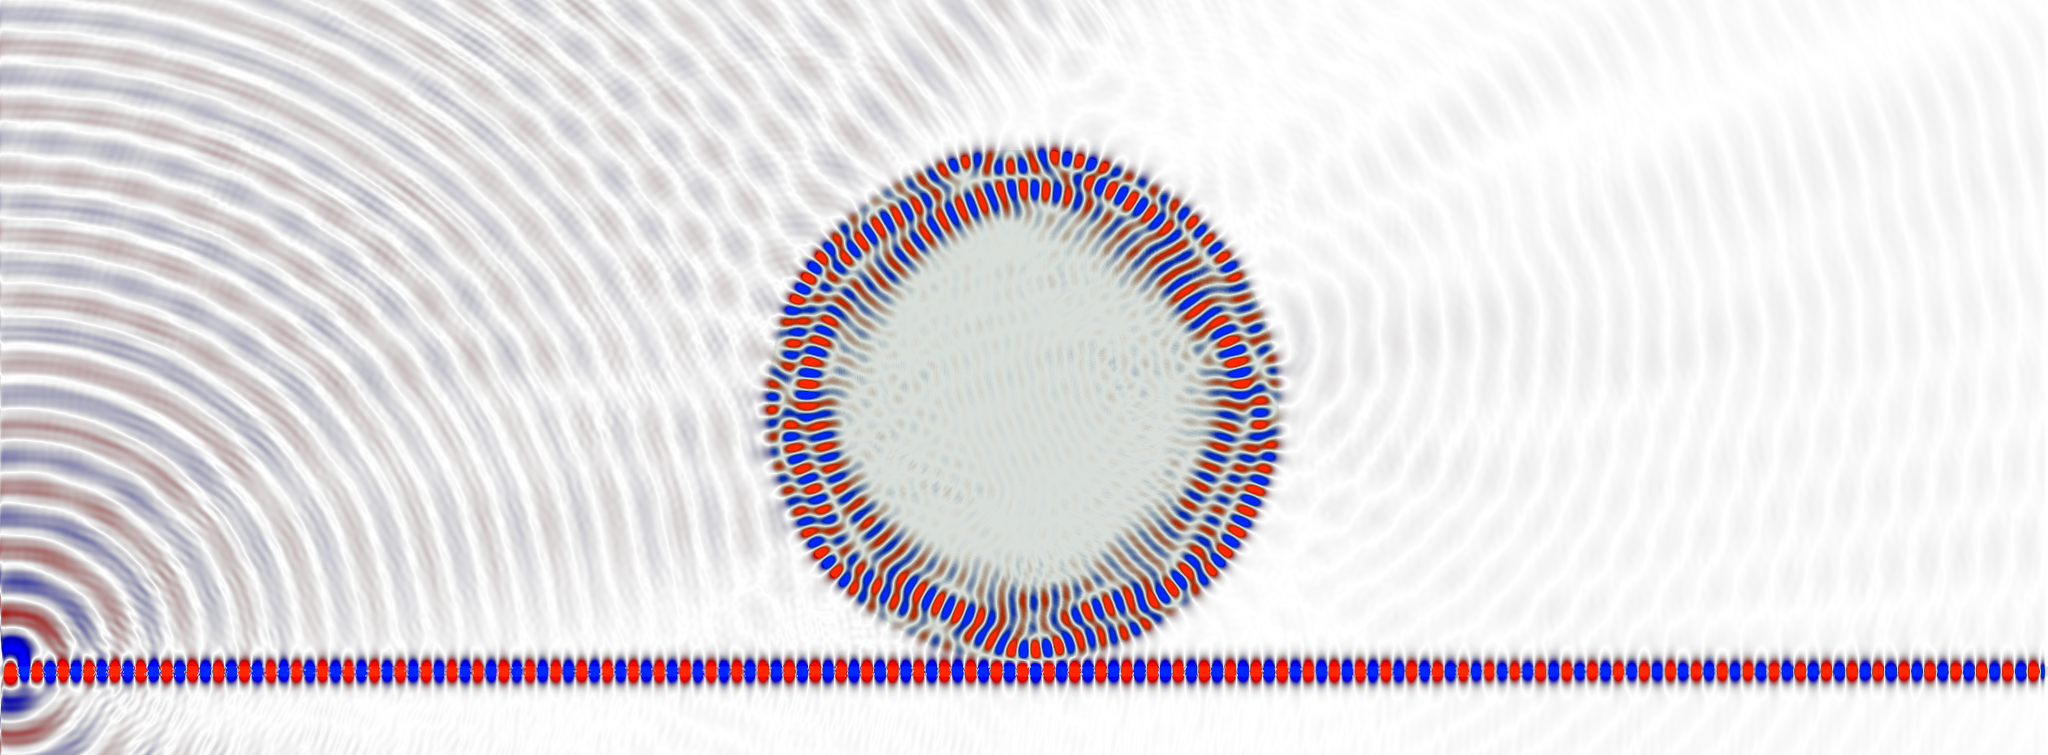
\includegraphics[  width=15cm,
	height=6cm,
	keepaspectratio]{visualizer-wgm.png}
	\caption{2D Whispering Gallery Mode Sensor}
	\label{fig:wgm}
\end{figure}


\section{Modeling approach}

For simplicity, models are defined in any of a number of standard 32-bit color image formats.

In a 32-bit per pixel image, each color has 8-bit red, green, blue and alpha values. As mentioned in the model processor (\autoref{sec:modelProcessor}) section, each component is used to indicate some data about a given point in the simulation domain:

\begin{table}[h!]
	\centering
	\caption{Color component usage}
	\label{tab:modelColorComponentUsage}
	\begin{tabular}{l | l | l}
		Component	& Meaning & Interpretation\\
		\hline															 \\
		Red		& Source 				& normalizezd wavelength of the source \\
		Green	& Dielectric			& $\epsilon_r = green * \frac{\epsilon_{max}}{255.0}$) 	 \\		
		Blue	& Monitor				& ID of the monitor to which this texel belongs \\
		Alpha	& Reserved				& Reserved for future use. \\
	\end{tabular}
\end{table}

Whenever a non-zero blue (monitor) value is encountered, it is used as an "ID" of a monitor. If the given ID has not yet been encountered, a new monitor is created. Texels with the same blue are added to the corresponding monitor. This allows monitors to be of any shape or size.
 
Using a tool such as Adobe Photoshop or Microsoft Paint, the user can specify all necessary data - sources, monitors and dielectric - in an intuitive fashion. Alternatively, these bitmaps could be generated by a custom tool which would voxelize a CAD model, assigning color components based on the model's metadata or object properties. 

A significant advantage of this approach over the CSG method used in Meep is that all constructs - sources, monitors and dielectric - can be of any shape that can be drawn in a bitmap. In theory, any 3D voxel-based painting application could be used to build models in higher dimensions. 

\begin{figure}[H]
	\centering
	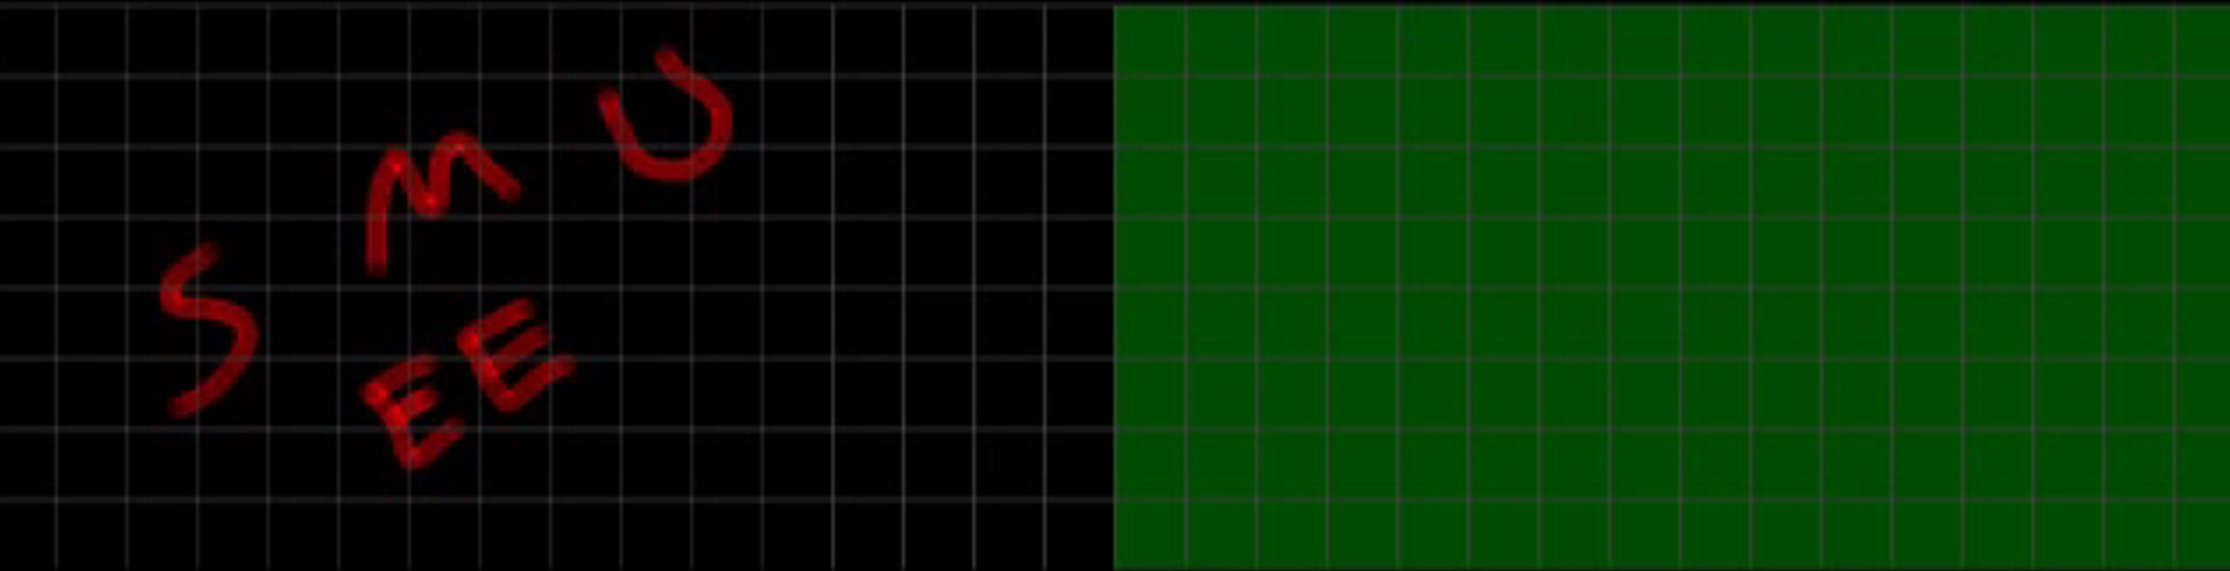
\includegraphics[  width=15cm,
	height=6cm,
	keepaspectratio]{arbitrary-source-shape.png}
	\caption{Arbitrarily-shaped source (Red pixels)}
	\label{fig:arbitrarySource}
\end{figure}

\begin{figure}[H]
	\centering
	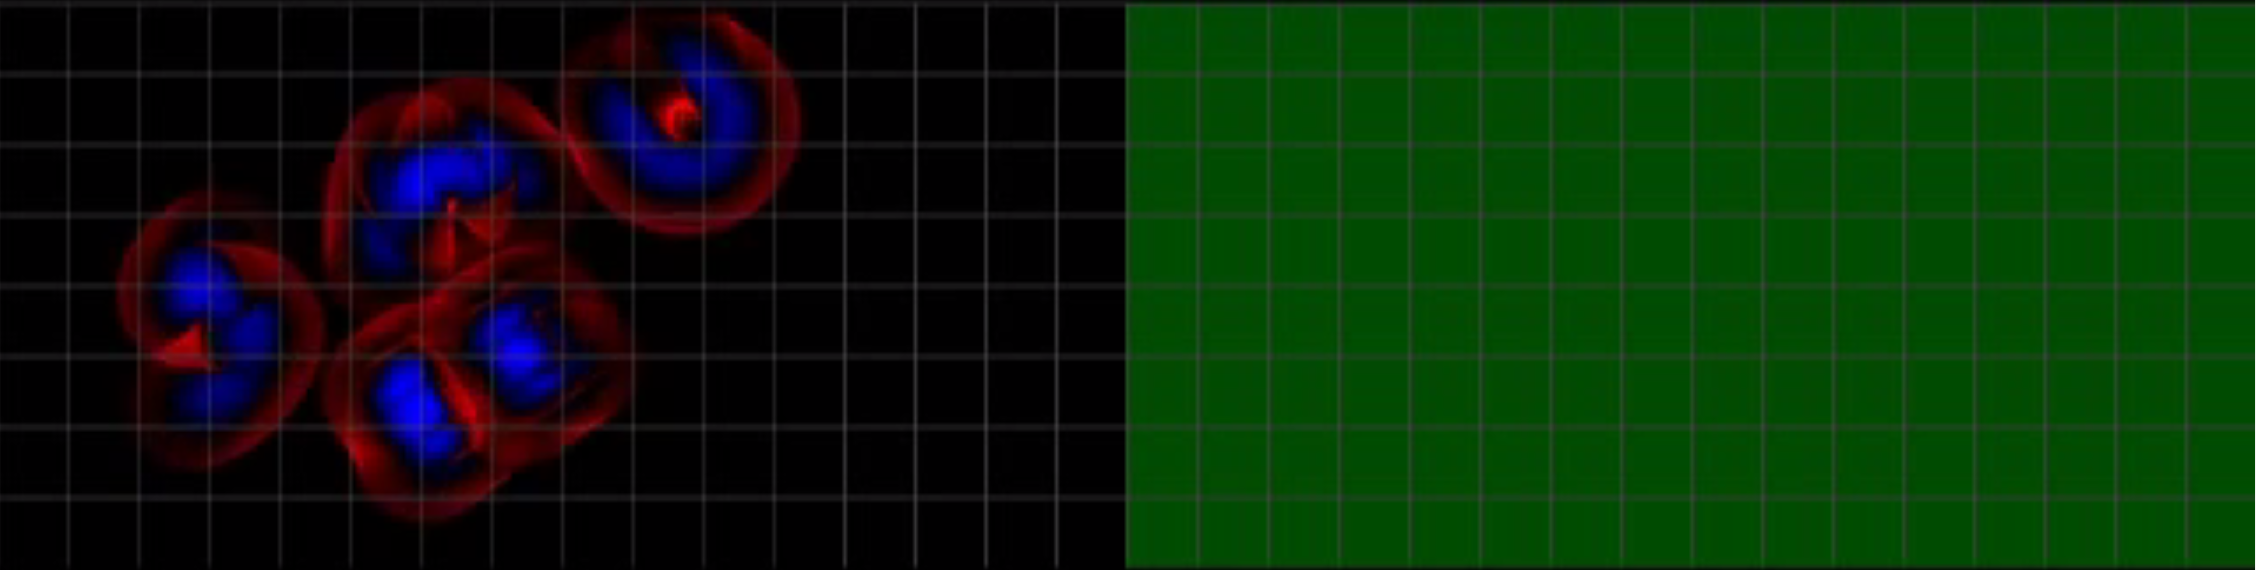
\includegraphics[  width=15cm,
	height=6cm,
	keepaspectratio]{arbitrary-source-shape2.png}
	\caption{Arbitrarily-shaped source after 20 frames}
	\label{fig:arbitrarySource2}
\end{figure}

\begin{figure}[H]
	\centering
	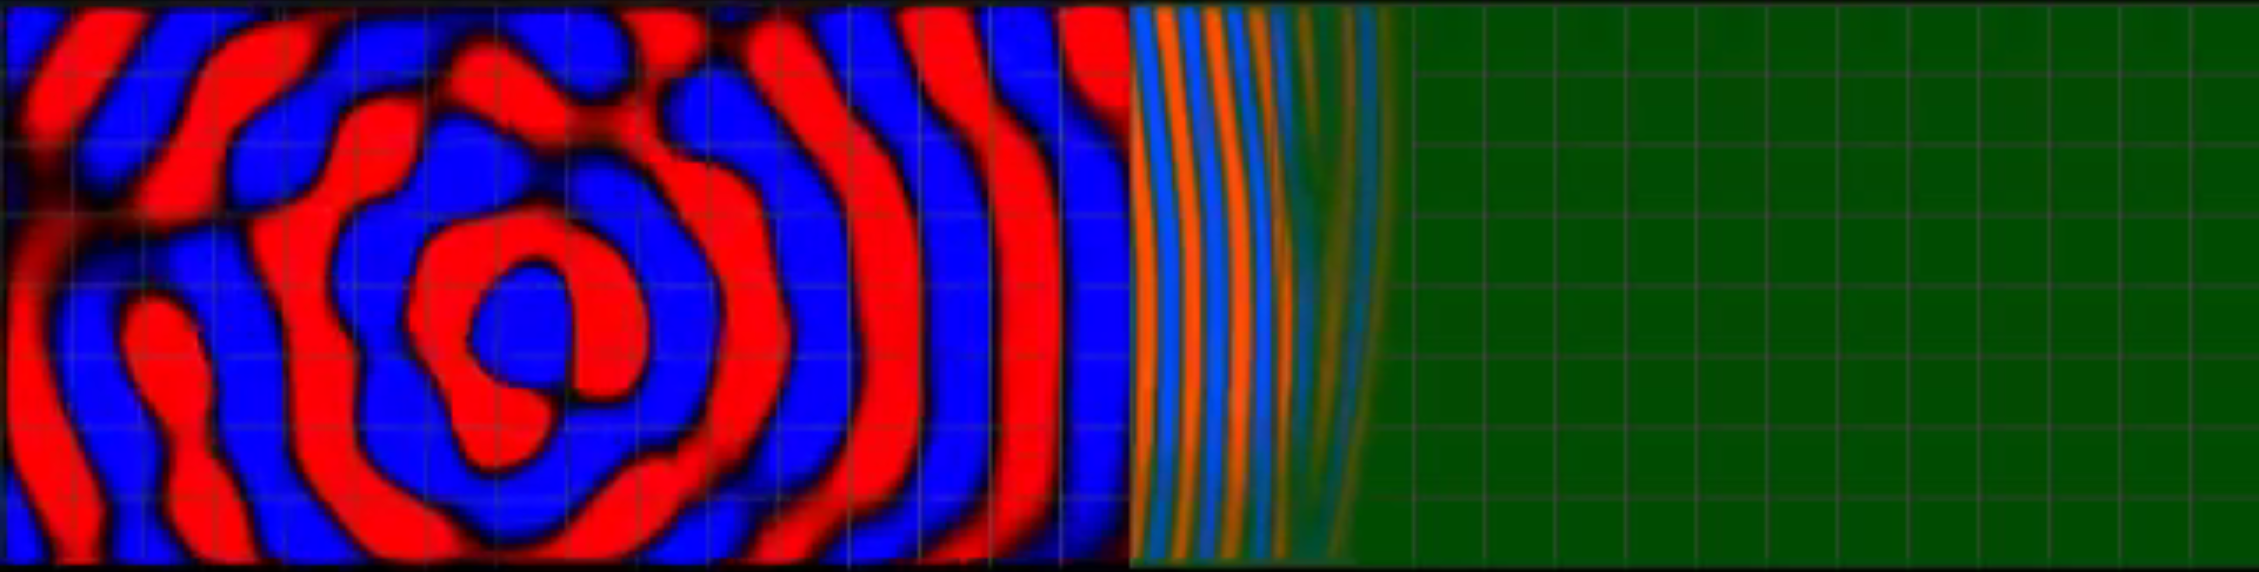
\includegraphics[  width=15cm,
	height=6cm,
	keepaspectratio]{arbitrary-source-shape3.png}
	\caption{Arbitrarily-shaped source after 100 frames}
	\label{fig:arbitrarySource3}
\end{figure}

\section{Testing and Validation Methodology}

In order to validate the functionality of the simulator, a 2D $TM_Z$ simulation was executed.

\begin{figure}[H]
	\centering
	
\includegraphics[  width=15cm,
	height=6cm,
	keepaspectratio]{plane-wave-test-model.png}
	\caption{$TM_Z$ Test Model with Plane Wave.}
	\label{fig:plane-wave-test-model}
\end{figure}

As can be seen in \autoref{fig:plane-wave-test-model}, the simulation includes a plane wave source (red line), monitors for incident and transmitted waves, and a slab of dielectric with $\epsilon_R = 9$. An additional monitor at the source location is not clearly visible due to it's relatively low ID (B = 5).

The simulation was first run with $\epsilon_R = 1$ to to record the incident magnitude in absenceof any reflective interfaces.

The simulation was then run with $\epsilon_R = 9$ to record combined incidence and reflection, as well as transmittance within the dielectric.

In a post-processing step, the reflective magnitude was found by subtracting the incident wave magnitude obtained from the first simulation from the combined incidence and reflection magnitudes obtained from the second simulation.


\
\begin{equation}
|R| = |I + R| - |I|
\end{equation}


Validation was performed by comparing the theoretical Fresnel coefficients for the test model with the time-averaged power (RMS) recorded during the simulation.

\subsection{Analytical Result}

In the test configuration, a normalizezd ($\lambda = 1$) $TM_Z$ plane wave is normally incident upon a dielectric interface with $\epsilon_R = 9$. 


\begin{figure}[H]
	\centering
	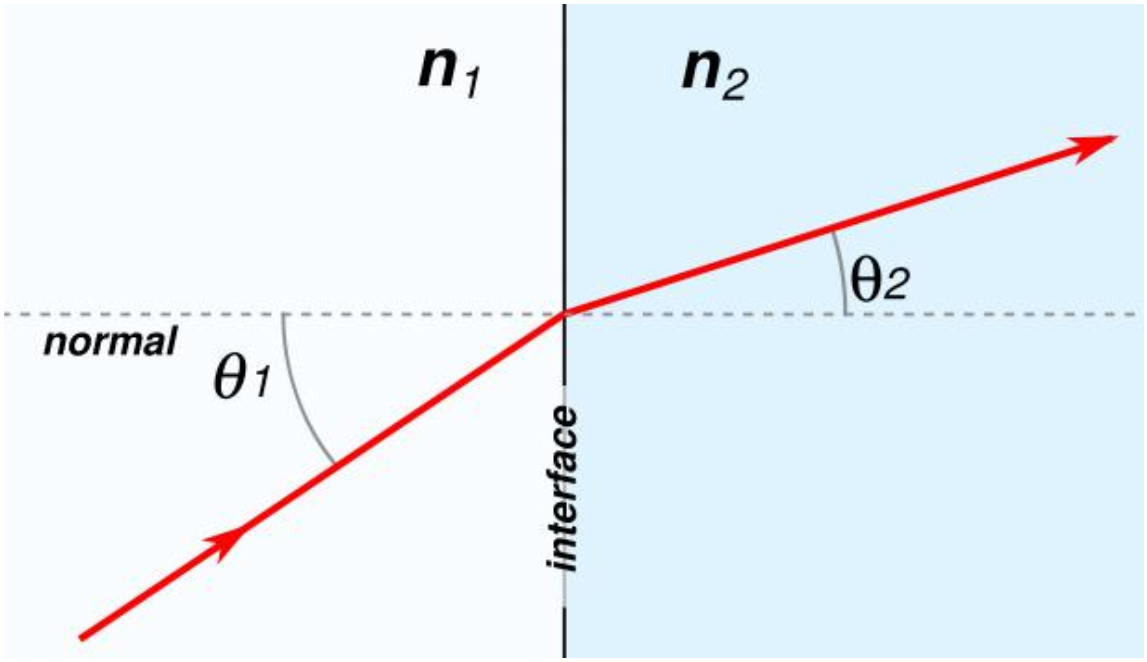
\includegraphics[  width=15cm,
	height=6cm,
	keepaspectratio]{snells-law.png}
	\caption{Snell's Law}
	\label{fig:snellslaw}
\end{figure}

Snell's Law states that the ratio of the refractive indices of the media at an interface, along with the angle of incidence, determine the angle of transmittance. (See \autoref{fig:snellslaw}) 

Mathematically, this relationship may be expressed as

\begin{equation}
n_1 \sin \theta_1 = n_2 \sin \theta_2
\end{equation}

In the testmodel, the index $n_2$ is calculated using the formula:

\begin{equation}
n = \sqrt{\epsilon_0 \epsilon_R \mu_0 \mu_R}
\end{equation}

In our simulator, $\epsilon_0$ and $\mu_0$ are normalized to 1. Similarly, in the non-magnetic media used in this case, 
\begin{equation}
\mu_R = 1
\end{equation}

Using our test value of $\epsilon_R = 9$ gives 

\begin{equation}
n_2 = \sqrt{9} = 3
\end{equation}

For a normally-incident plane wave, the incident and refraction angles are

\begin{equation}
\theta_I = 0
\end{equation}

and

\begin{equation}
\theta_T = 0
\end{equation}

Evaluating the Fresnel equations for the reflection and transmission of a $TM_Z$ wave,

\begin{equation}
r = \frac{n_2 \cos \theta_I - n_1 \cos \theta_T}{n_1 \cos \theta_T + n_2 \cos \theta_I}
\end{equation}
\begin{equation}
t = \frac{2 n_1 \cos \theta_I}{n_1 \cos \theta_T + n_2 \cos \theta_I}
\end{equation}

gives the coefficients:

\begin{equation}
r = \frac{3 * 1- 1 * 1}{1 * 1 + 3 * 1} = \frac{1}{2}
\end{equation}
\begin{equation}
t = \frac{2 * 1 * 1}{1 * 1 + 3 * 1} = \frac{1}{2}
\end{equation}

In this case, given a dielectric constant $\epsilon_R  = 9$, the reflection and transmission coefficients are equal.

\subsection{Numerical Result}

The observed steady-state output of the simulation for the baseline case ($\epsilon_R = 1$) is show in \autoref{fig:planewavefreespace}.

\begin{figure}[H]
	\centering
	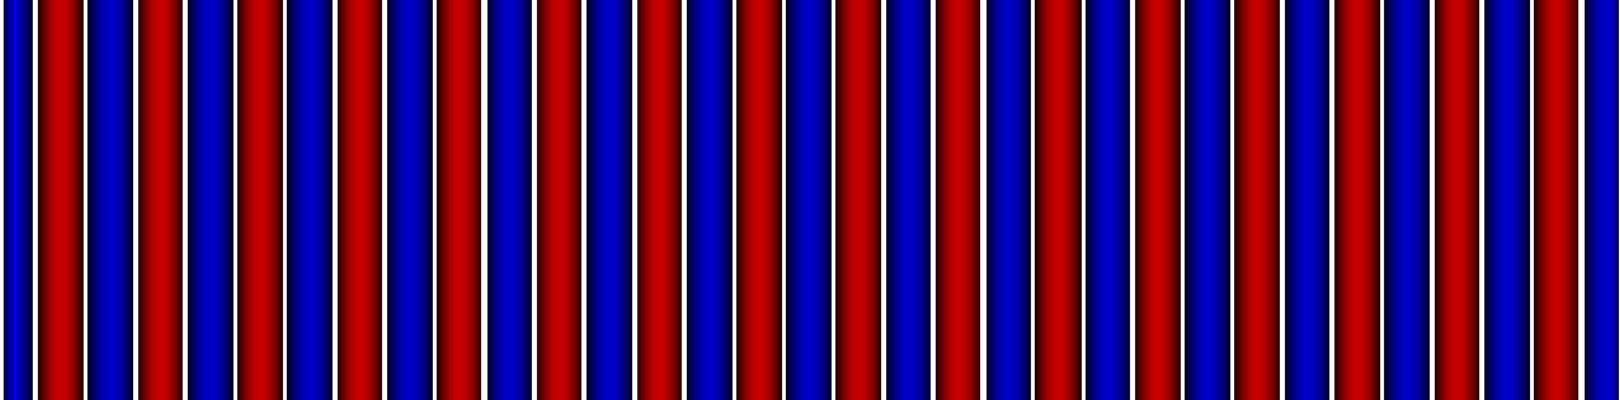
\includegraphics[  width=15cm,
	height=6cm,
	keepaspectratio]{plane-wave-free-space.png}
	\caption{Plane wave with $\epsilon_R = 1$}
	\label{fig:planewavefreespace}
\end{figure}

The time-averaged (RMS) numerical output for the incident and transmitted monitors is

\begin{figure}[H]
	\centering
	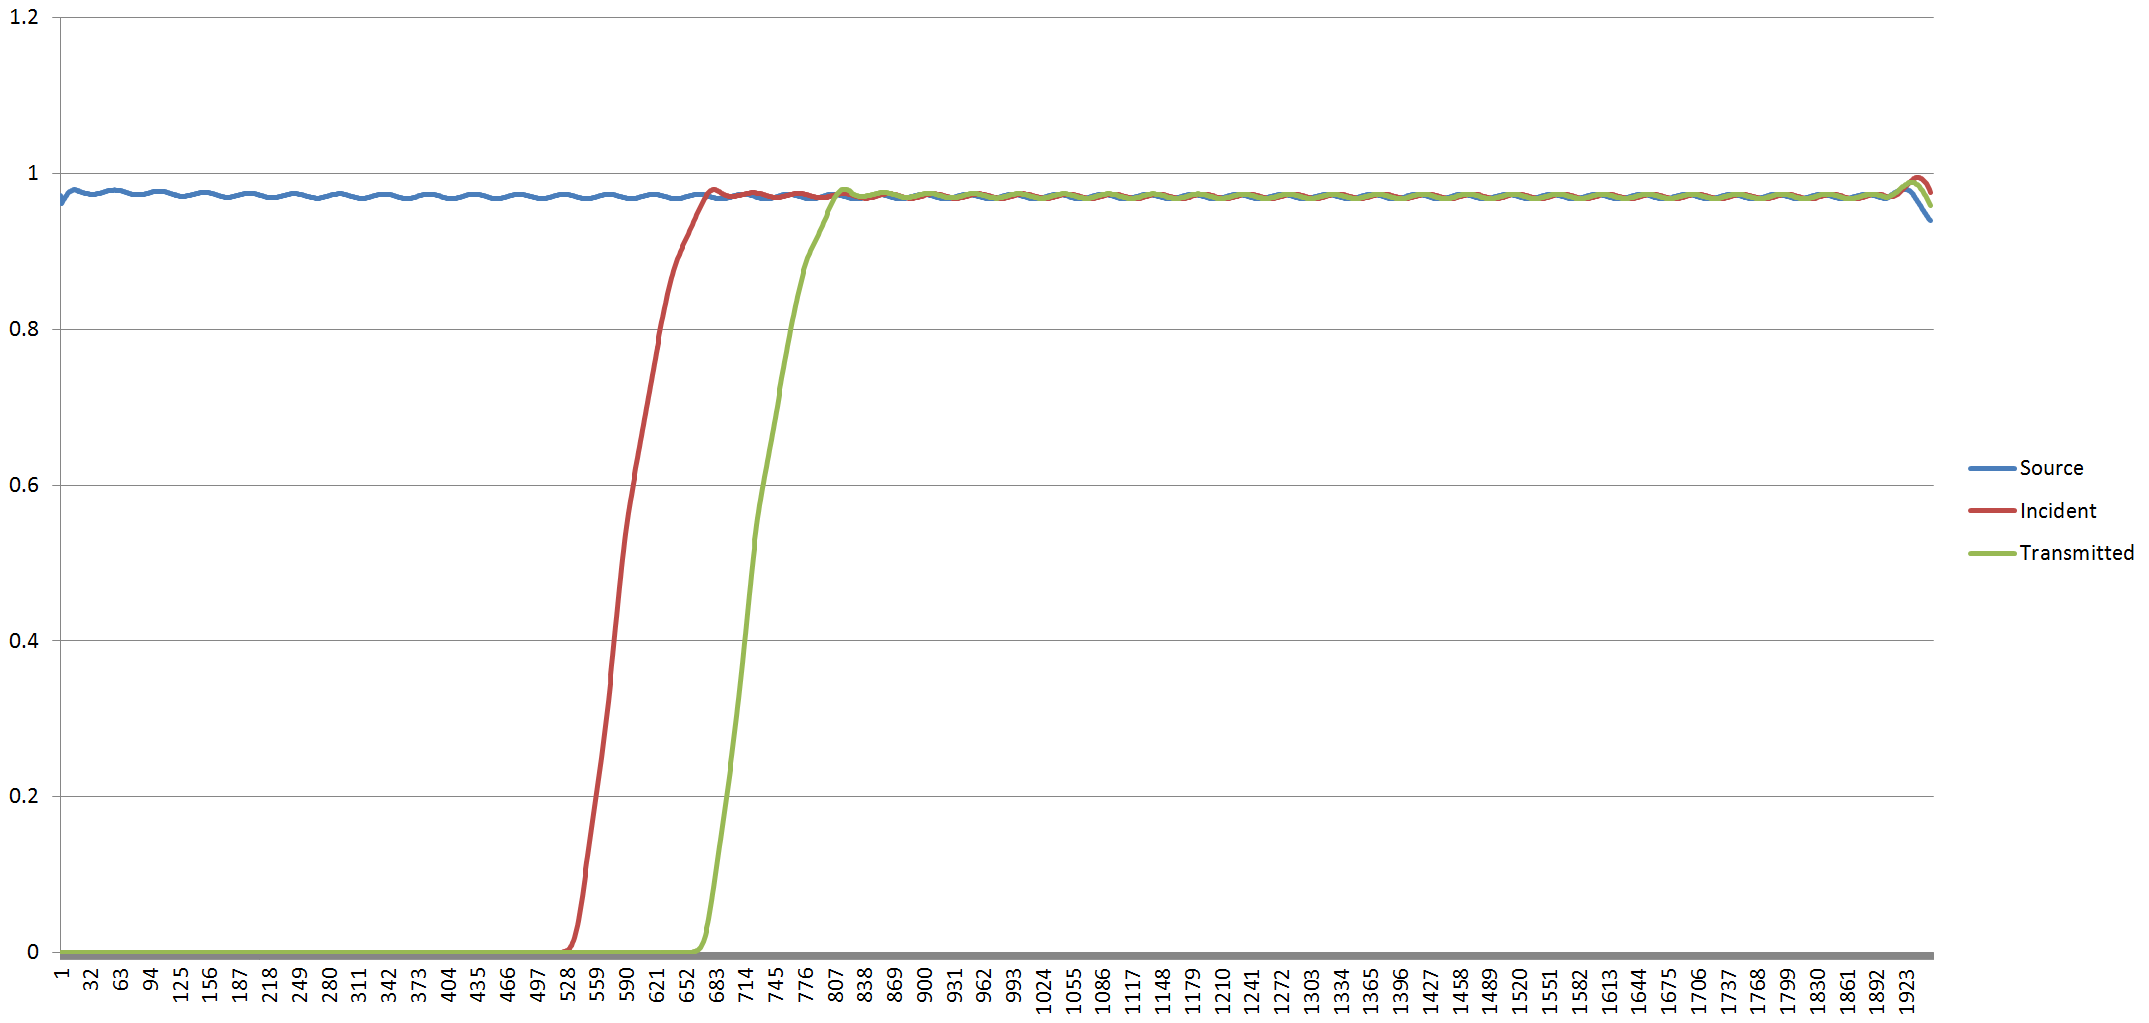
\includegraphics[width=\textwidth,
	keepaspectratio]{pw-time-averaged-output.png}
	\caption{Time-averaged (RMS) output in free space $\epsilon_R = 1$}
	\label{fig:planewaveRMSinFreeSpace}
\end{figure}

As expected, the incident and transmitted magnitudes equal the source magnitude, offset by the time it takes for the wave to propagate from the source to themonitors.

The observed output of the same simulation, executed with dielectric constant $\epsilon_R = 9$,

\begin{figure}[H]
	\centering
	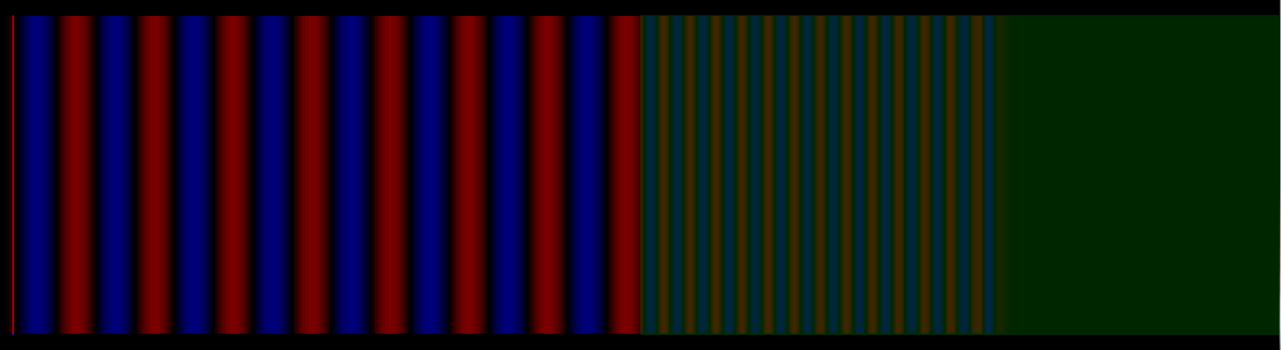
\includegraphics[width=\textwidth,
	keepaspectratio]{pw-epsilon-9.png}
	\caption{Steady state with $\epsilon_R = 9$}
	\label{fig:pwEpsilon9}
\end{figure}

Note the difference in $\lambda$ once the wave enters the dielectric (green area). This simulation produces the following raw output:

\begin{figure}[H]
	\centering
	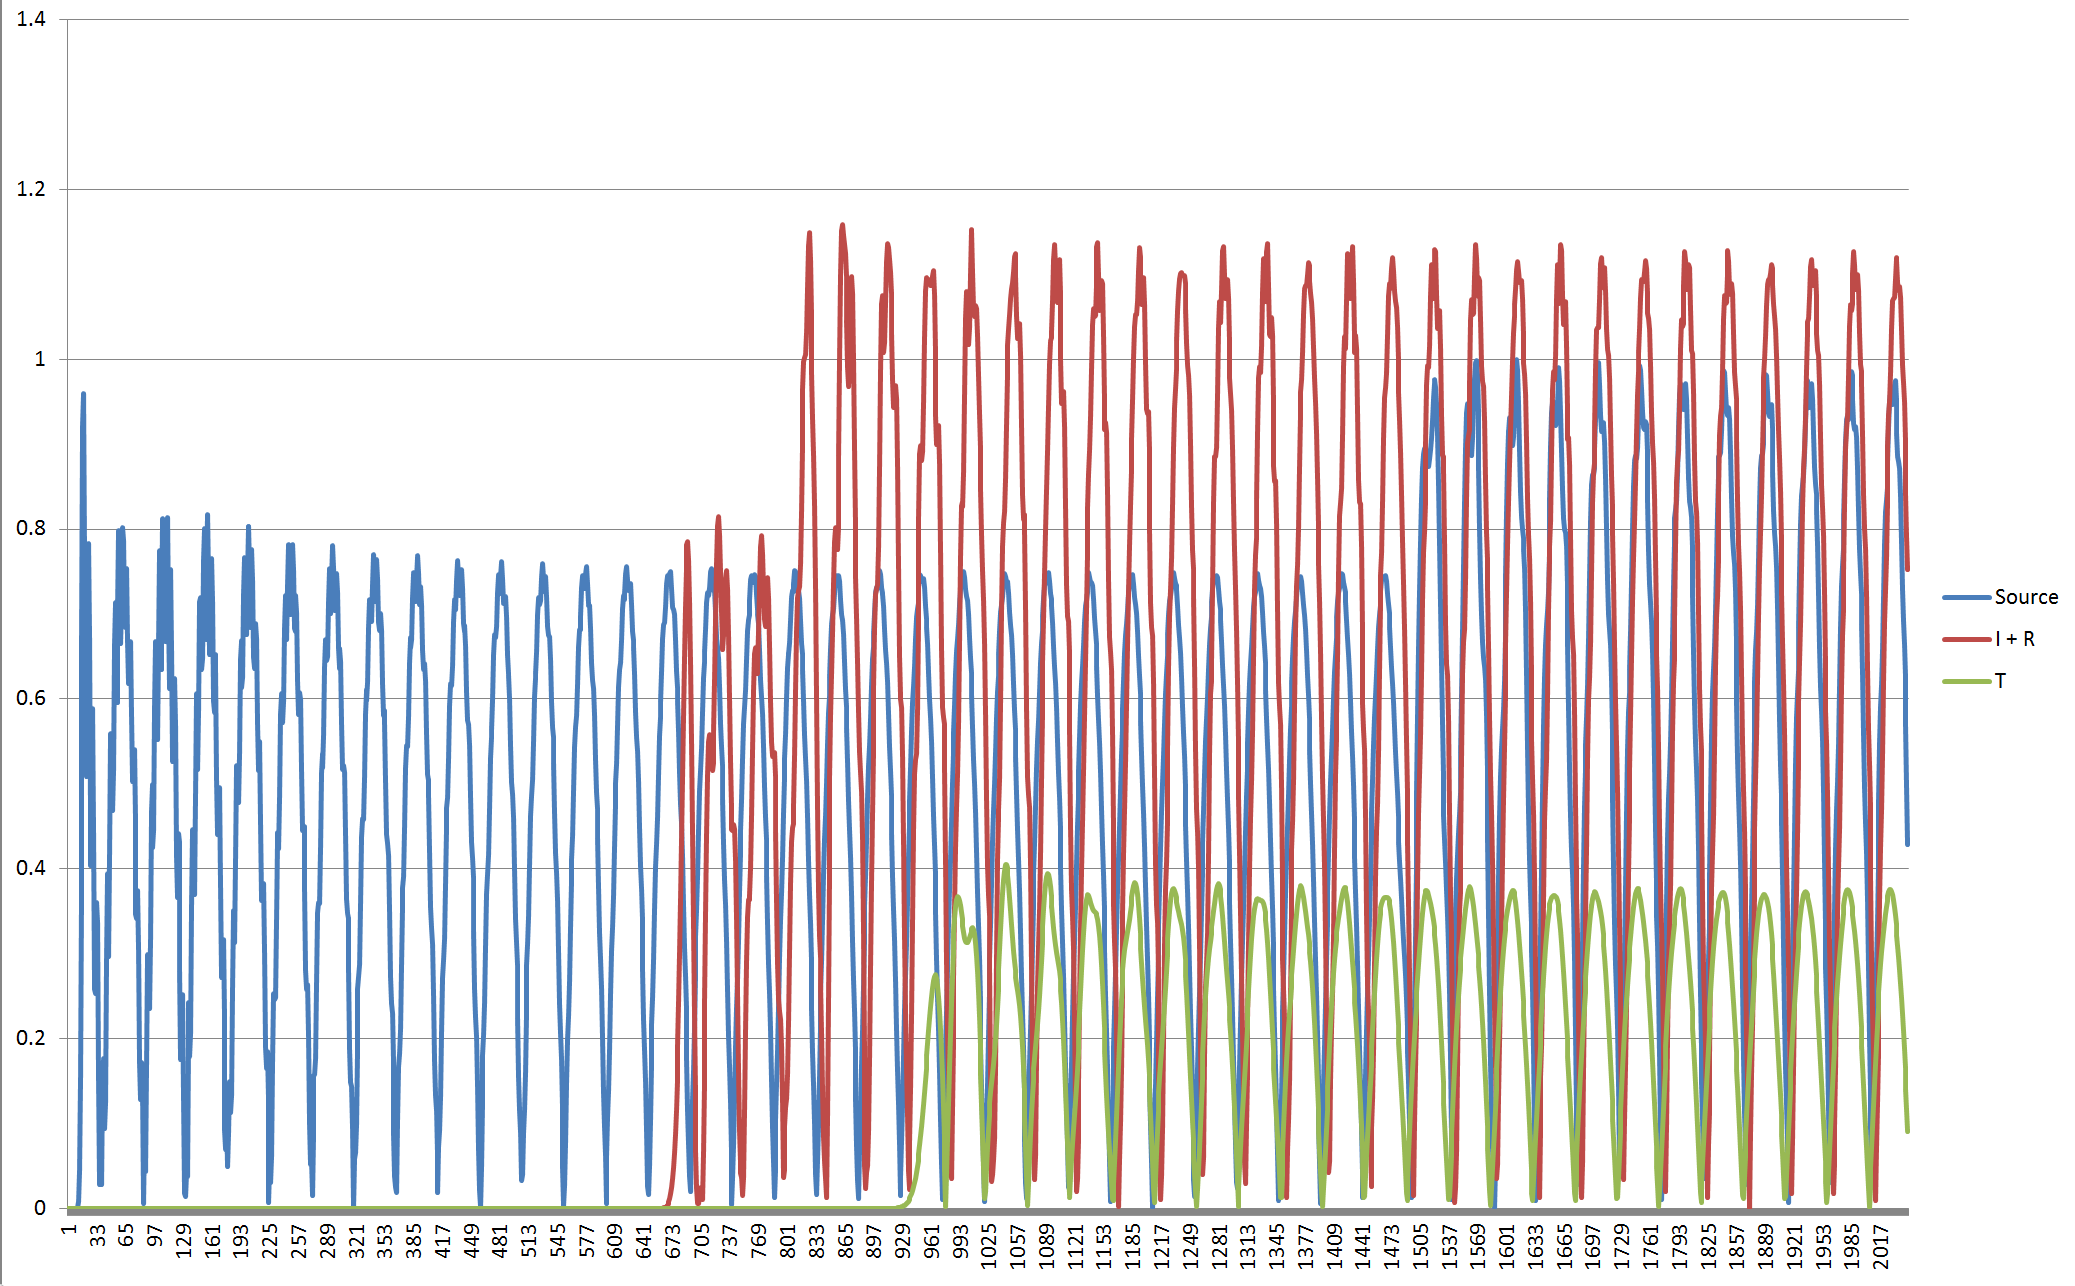
\includegraphics[width=\textwidth,
	keepaspectratio]{pw-epsilon-9-raw.png}
	\caption{Raw monitor output with $\epsilon_R = 9$}
	\label{fig:pwEpsilon9Raw}
\end{figure}

The time-averaged power for the monitors:

\begin{figure}[H]
	\centering
	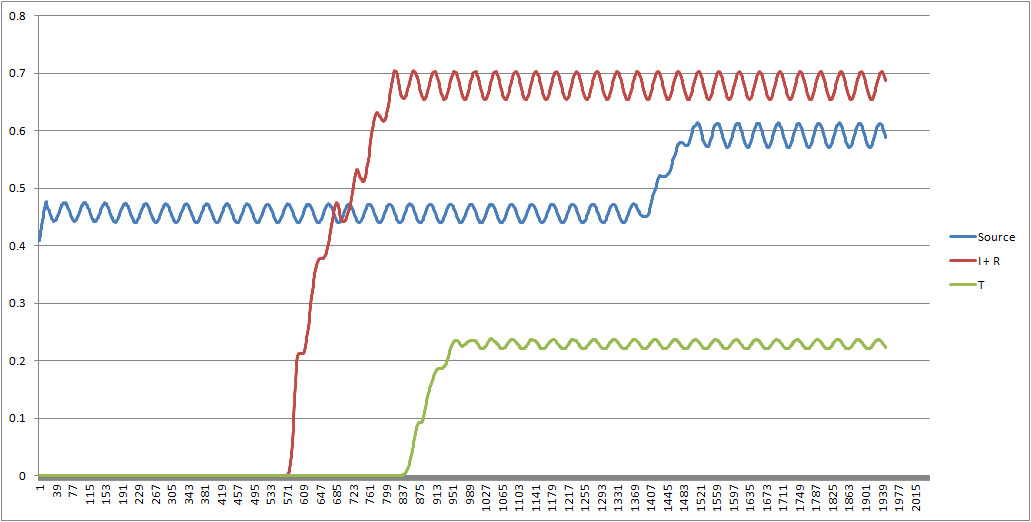
\includegraphics[width=\textwidth,
	keepaspectratio]{pw-epsilon-9-rms.png}
	\caption{RMS output with $\epsilon_R = 9$}
	\label{fig:pwEpsilon9RMS}
\end{figure}

Subtracting the incident magnitude from the simulation with $\epsilon_R = 1$ from the second simulation with $\epsilon_R = 9$ gives the following normalized result:

\begin{figure}[H]
	\centering
	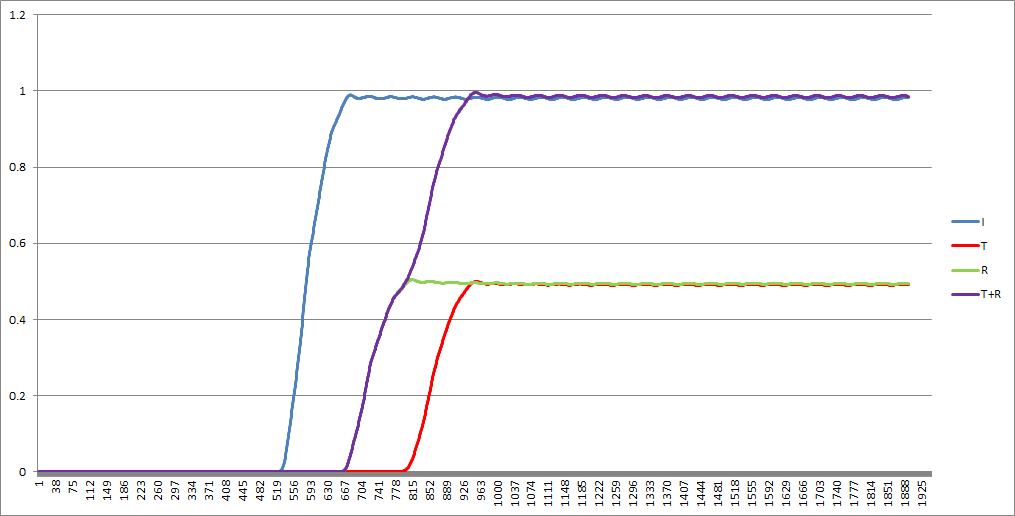
\includegraphics[width=\textwidth,
	keepaspectratio]{pw-epsilon-9-tir-power.png}
	\caption{Normalized output with $\epsilon_R = 9$}
	\label{fig:pwEpsilon9Normalized}
\end{figure}

In this case, the average of each of the relevant values are determined to be:

\begin{center}
$I_{avg} = 0.96214...$

$T_{avg} = 0.4882...$

$R_{avg} = 0.484...$
\end{center}

Conservation of energy requires that the sum of the transmitted (T) and reflected (R) magnitudes equals the incident magnitude (I).

\begin{equation}
I = T+ R
\end{equation}

The computed error of the computational result is

\begin{equation}
I_{error} = |\frac{I_{avg} - (T_{avg} + R_{avg})}{I-{avg}}|
\end{equation}

Gives

\begin{center}
	\begin{math}
	|\frac{0.9621-(0.4882 + 0.4843)}{0.9621}| = 1.011\%
	\end{math}
\end{center}

Comparing to the analytically-derived Fresnel coefficients,

\begin{equation}
T = \frac{T_{avg}}{I_{avg}} = \frac{0.4882219...}{0.962135...} = 0.507
\end{equation}
\begin{equation}
R = \frac{R_{avg}}{I_{avg}} = \frac{0.484332......}{0.962135...} = 0.503
\end{equation}

The error contribution of each component may be expressed as:

\begin{equation}
T_{error} = |1 - \frac{T_{computed}}{T_{analytical}}| = |1 - \frac{0.507}{0.5}| = 1.4\%
\end{equation}
\begin{equation}
R_{error} = |1 - \frac{R_{computed}}{R_{analytical}}| = |1 - \frac{0.503}{0.5}| = 0.6\%
\end{equation}

Careful analysis of different simulation results indicates that this error is due to floating-point precision errors. As every frame output depends on the state of the previous frame, small errors are compounded over time. 






\chapter{Results} \label{ch:conclusions}


Metrics were calculated using domain sizes ranging from 128x64 to 8192x4096 over 5000 frames. (In this case, a frame represents a complete time step wherein both E and H fields are updated.) For benchmarking purposes, the visualizer was disabled.

\begin{figure}[H]
	\centering
	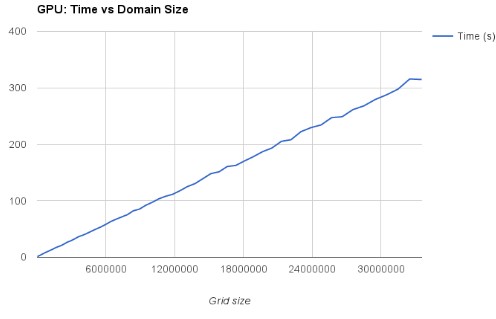
\includegraphics[width=\textwidth,
	keepaspectratio]{gpu_time_vs_domain_size.png}
	\caption{GoLightly: seconds for 5000 frames with the given domain size}
	\label{fig:gpuTimeVsDomainSize}
\end{figure}

As expected, As the number of computational cells in the simulation domain increases, the required computation time increases linearly.

\begin{figure}[H]
	\centering
	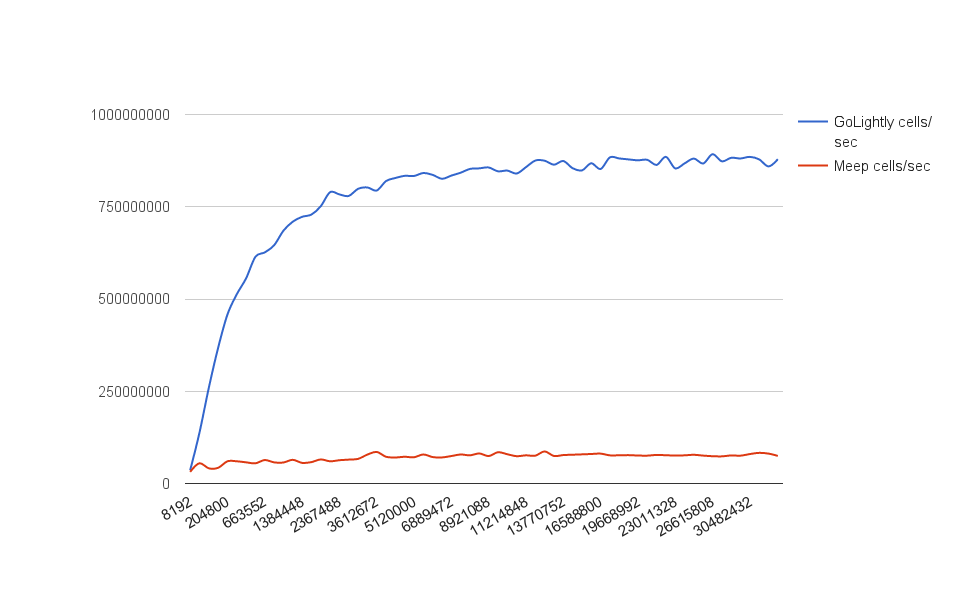
\includegraphics[width=\textwidth,
	keepaspectratio]{cells-per-second.png}
	\caption{GoLightly: Completed E and H updates per second}
	\label{fig:gridSizeVsComputeTime}
\end{figure}

Note that the total throughput (represented in the following figure as “cell” operations per second) increases dramatically as the domain size increases, until the point where GPU initialization overhead is outweighed by computation time.

Comparing to Meep:

\begin{figure}[H]
	\centering
	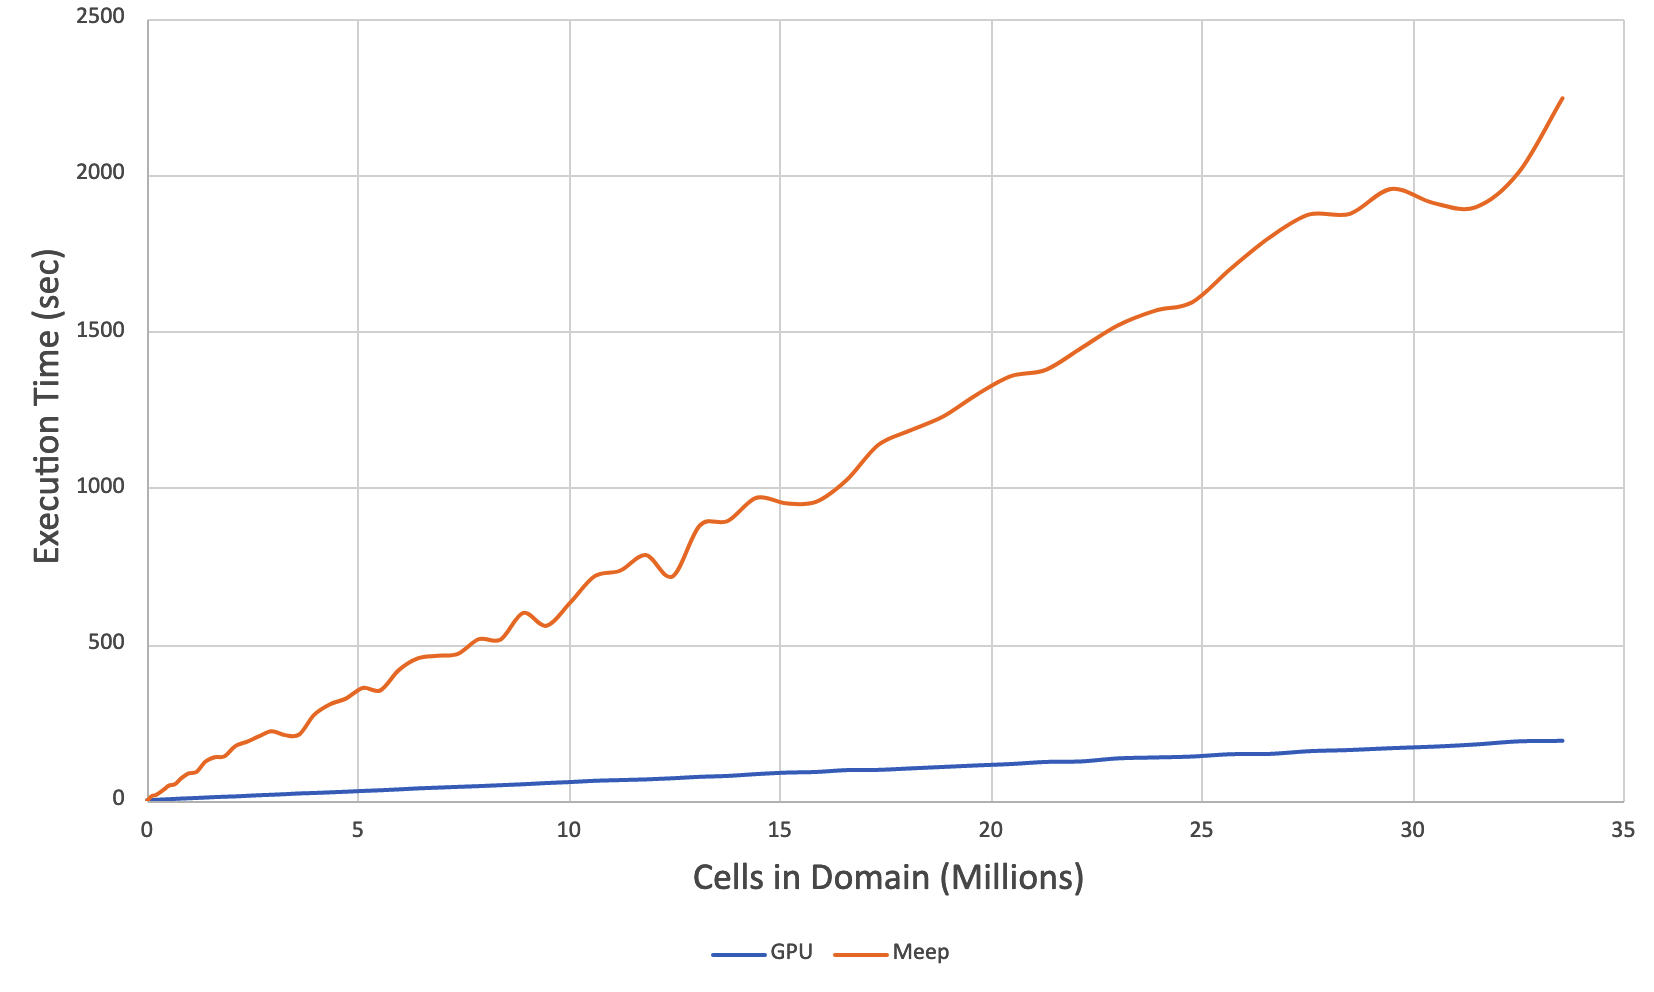
\includegraphics[width=\textwidth,
	keepaspectratio]{gpu-vs-meep.png}
	\caption{GoLightly vs Meep}
	\label{fig:gpuVsMeep}
\end{figure}

\begin{figure}[H]
	\centering
	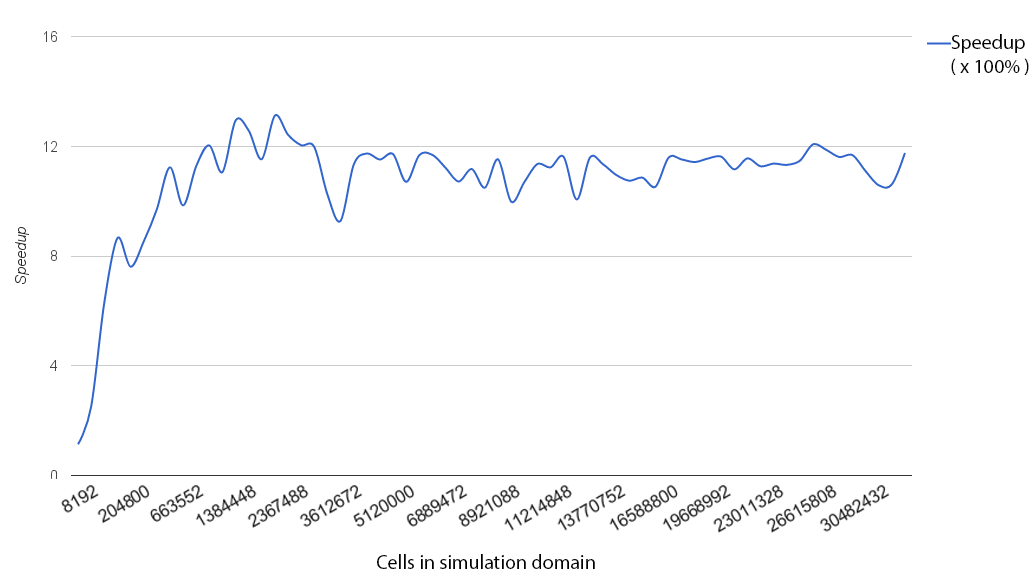
\includegraphics[width=\textwidth,
	keepaspectratio]{gpu-vs-meep-speedup.png}
	\caption{Speedup - Meep Time / GoLightly Time}
	\label{fig:gpuVsMeepSpeedup}
\end{figure}

This gives us a speedup ranging from 1.2 to 12, depending on the domain size. At lower resolutions, the overhead of initializing assets on the GPU can take more time than the simulation. In that case, a CPU-based simulation may outperform the GPU solution.

\section{Optimization and Enhancements}

Although a 1200\% speed increase is significant, there is much room for improvement. 

GPUs provide different memory spaces that vary in size and access speed. In addition to global device memory, each warp (group of 32 threads sharing an ALU) has shared memory\footnote{Shared memory is physically local to the ALU and accessible by all threads within the warp.} and local memory\footnote{Each thread has local memory which is not accessible to any other thread}.

While global memory is the most flexible and plentiful - typically on the order of gigabytes on current generation hardware - it is also the slowest. 

Shared memory is roughly equivelant to a CPU's L2 cache. It can be used for intra-thread synchronization and resource sharing. It is significantly faster than global memory.

Finally, local memory - similar to a CPU L1 cache - provides thread-local storage. Local memory provides the lowest latency of all of the memory spaces.

In its current form, GoLightly makes little use of shared or local memory. Modifying the application to take advantage of those may improve performance.









\chapter{Conclusions} \label{ch:conclusions}

Using the GoLightly simulator, we have shown a speedup potential of up to 12 times that achieved by CPU-based solutions.

\section{Usability}

Although the software, in its current state, may not be suitable for production, it is clear that a GPU-based approach promises substantially improved performance. This results in increased productivity and, ultimately, better products. Eliminating the script-only modeling approach enforced by other packages makes utilization of this application significantly easier, and therefore accessible to a wider audience.

\section{Future Work}

The vastly-improved performance afforded by this system presents some interesting opportunities:

\subsection{GoLightly Improvements}

Care must be taken during the design process to avoid nonsensical monitor configurations, such as disjoint or outlying pixels, or inconsistent thickness due to shape aliasing. A model validation step could correct model errors. Sub-pixel averaging would increase effective domain resolution near dielectric boundaries and reduce structure aliasing. 

\clearpage

\subsection{Genetic Algorithms}
Genetic algorithms\cite{Mitchell:1998:IGA:522098}\cite{Goldberg:1989:GAS:534133}  are intended to let software take over a part of the design process. By defining a problem in terms of a number of inputs and creating a fitness function, an application can potentially test many different designs and use a feedback loop to suggest new permutations. This approach has been shown to be successful in such diverse fields as antenna design\cite{globus2006automated}, turbine design\cite{MOSETTI1994105} and pharmaceutical research\cite{Chi:2009:MLG:1651932.1652161}. 

A fast FDTD implementation will facilitate application of this technique to optical circuit design. By defining a problem domain in terms of desired package size, available inputs, allowed waveguide shape and dielectric properties, and designing an appropriate fitness function, software will be able to rapidly evaluate different designs and suggest new permutations. This may also dramatically reduce time-to-market and reveal new research avenues. 


\subsection{Arbitrary Domain Shape and PML Sinks}
Given the flexible voxel-based model definition used in GoLightly, it becomes possible to create completely arbitrary domain shapes. Non-rectangular domains with PML "sinks" at any desired position within the domain would allow the designer to more tightly fit the computational domain to the circuit in question while ignoring irrelevant or uninteresting areas.

PML sinks would potentially increase performance by reducing memory requirements. If large sections of a domain could be surrounded by PML, those sections are effectively disjoint from the rest of the domain and therefore may be ignored and, in fact, removed from the simulation. 

Although the current implementation treats the domain as a regular grid of identical blocks, this is a programming convenience and is not dictated by the FDTD algorithm.

In addition to non-rectangular domains, non-rectangular cell shapes could improve simulation fidelity. For example, in a $TM_Z$ simulation, each $E_Z$ component could be treated as the center of a hexagonal grid cell. As such, it would be updated using three derivatives instead of two. While this would increase the computation requirement for each $E$ cell by roughly 50\% (in a two-dimensional domain), the improved fidelity may justify the cost in experiments where improved accuracy is valuable. Inclusion of the afore-mentioned PML sink capability could offset this cost. 

\subsection{Load Balancing}
Although we have shown that a GPU implementation of FDTD can outperform a CPU implementation, CPUs should not be ignored. It is possible to divide computational load between the CPU and GPU in a manner analagous to that used to distribute load between machines in a cluster. 

When combined with load balancing between separate machines, this technique would allow the GPU to act as an additional cluster node, providing a more ideal solution which, rather than trading a CPU for a GPU, utilizes the power of both. 

\subsection{Machine Learning}
A high-speed simulator such as GoLightly may facilitate application of machine learning algorithms to accelerate FDTD even more. ML systems excel at identifying complex relationships and patterns. In theory, one could present simulation parameters such as waveguide architecture and composition and source wavelengths as a set of inputs into a multi-layer neural network, while simulation output is used to evaluate the fidelity of the network's predicted output. 

A trained network may be able to predict a simulation's output with a degree of accuracy sufficient to inform the design iteration process.  The ability to rapidly execute simulations should make generation of the large quantities of training data required by ML networks more feasable than traditional CPU-based systems. 

\section{Final Words}

The field of general-purpose GPU computing offers potential yet to be realized in many of the areas where it shows the most promise. Leveraging this commonly available, underutilized resource will enable shorter, more robust design cycles, and facilitate exploration of more sophisticated waveguide architectures. 











%===================================================================
%   Appendices go here if no appendix, remove \StartAppendix
%===================================================================
%\StartAppendix %All chapters from this point are treated as appendices

%
\chapter{APPENDIX} \label{ch:table appendix}

%\vspace{-0.2in}

%\section{Description of GOY Shell Model Runs and Table}

%In most cases, we have forced the models in the first shell so that the inertial range %forms on the ultraviolet side.  However, in run 2 from Table \ref{table: app GOY table}, %we force in shell seven and observe an infra-red inertial range form.  Run 1 uses the %parameters of \cite{Yamada} originally used.  This run is used as a control and to %reproduce Pisarenko et. al. \cite{Pisarenko} work.  Run 2 is equivalent to Run 1 as far %as the parameters are concerned.  However, in this run, we force in shell 6.  As a %result, we see an infra-red inertial range.  We can apply the affine collapse to this %data as well. This result is of interest in the light of Carl Gibson idea that the true %cascade in turbulence is from small to large scales \cite{Gibson}. We start with small %forcing in Run 3.  Here, the forcing is small enough that the solution is quasi-periodic %and we have no inertial range.  We can observe this in the distribution of $u_n$.  In %this particular case, the points were located in a ring that was centered at the origin %(see Figure \ref{fig: circ symtrc}).   However, there is still circular symmetry about %the origin in this case.

%\begin{figure}[!htp]
%    \begin{center}
%        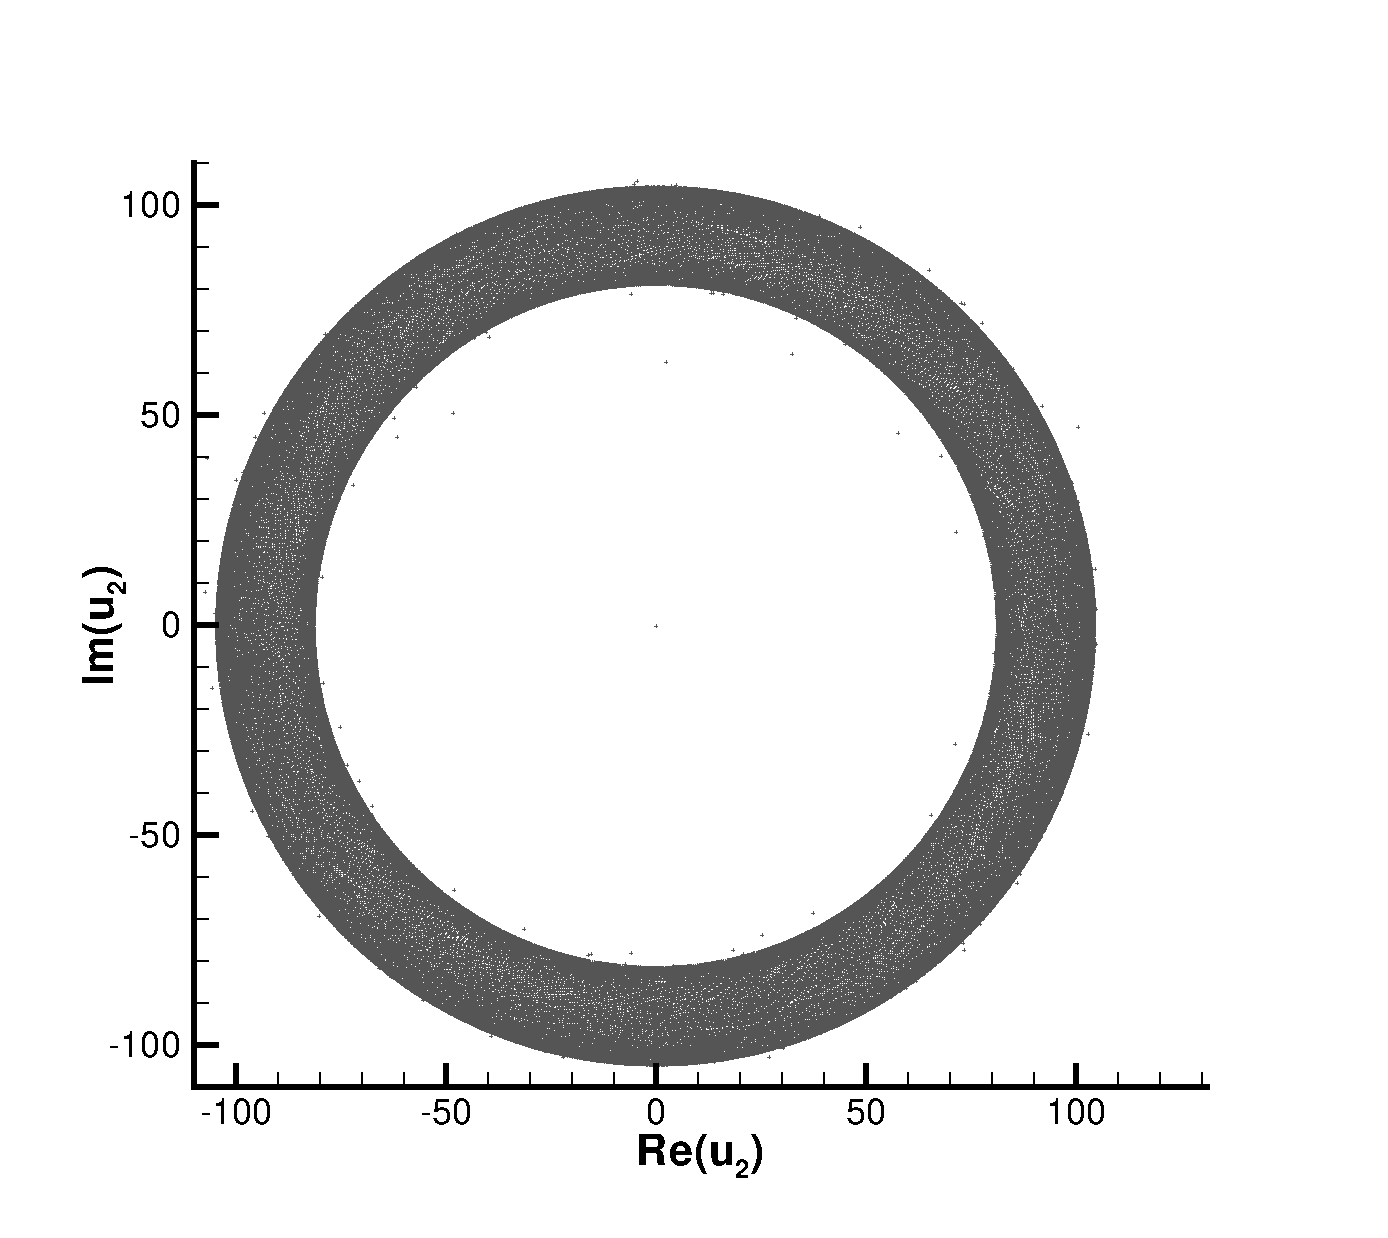
\includegraphics[width=4in]{ns_run10urui.eps}
%    \end{center}
%    \caption{Distribution of $u_i$. This plot displays the quasi-periodic nature of Run 3 %for shell 10 (eps file).} \label{fig: circ symtrc}
%\end{figure}



\section{Meep scripts}

The shell script shown in \autoref{meeptestsh} calls Meep in a loop, increasing the domain size from 128x64 cells (not including PML layers) to 8192x4096 cells in increments of 128x64 cells. 

\lstinputlisting[label=meeptestsh, language=bash,caption=Meep shell script]{meep-test.sh}


The Meep CTL code in \autoref{benchmarkctl} defines a simulation with a dielectric block with $\epsilon_{max}$ = 9. The simulation is run for 5000 frames for each domain size calculated in \autoref{meeptestsh}. During testing, the simulation is timed and the results are written to a CSV file for later analysis. 

\lstinputlisting[label=benchmarkctl,caption={Meep simulation CTL script}]{benchmark.ctl}

\section{GoLightly configuration}

Unlike Meep, GoLightly encodes most simulation parameters in an image file, typically generated in an image editing tool such as Adobe Photoshop or Microsoft Paint. That process is detailed in \autoref{sec:modelProcessor}. 

Additional parameters may be specified on the command line or in a text file. Valid options in the configuration text file are:

\begin{table}[h!]
	\label{golightlyConfig}
	\centering
	\caption{GoLightly Configuration}
	\label{tab:golightlyConfigTerms}
	\begin{tabular}{l | l}
		Option	& Description \\
		\hline
			model     & image file with encoded dielectric, source and monitor properties \\
			nogl      & disable OpenGL visualizer										  \\
			lambda    & source wavelength												  \\
			runlength & number of frames to run the simulation							  \\
			media     & $\epsilon_{max}$  for visualizer scaling								  \\
			output    & output path for images and numerical data						  \\
			paused    & start simulation paused, for debugging and timing				  \\
			width     & domain width if scaling model									  \\
			height    & domain height if scaling model									  \\
			benchmark & on / off to enable benchmarking									  \\
	\end{tabular}
\end{table}

For instance, one of the configuration files used while validating the simulator's functionality is shown below.

\begin{lstlisting}[caption={Samply GoLightly Configuration File},label={listing:sampleGolightlyConfig}]
model=coupler.psd
nogl
runlength=5000
benchmark=true
width=8192
height=4096
runlength=5000
lambda=10
media=9
\end{lstlisting}





%\input{app2.tex}

%===================================================================
%   Bibliography goes here
%===================================================================
\bibliographystyle{acm}
\nocite{*}
\bibliography{thesis}

\end{thesis}

\end{document}
